\documentclass{article}
\usepackage{fancyhdr}
\usepackage{hyperref}
\usepackage{enumerate}
\usepackage[backend=biber]{biblatex}
\addbibresource{references.bib}
\usepackage[top=2cm, bottom=2cm, right=2cm, left=2cm]{geometry}
\usepackage{graphicx}
\usepackage{subcaption}

\usepackage{listings}
\usepackage{color}
\definecolor{dkgreen}{rgb}{0,0.6,0}
\definecolor{gray}{rgb}{0.5,0.5,0.5}
\definecolor{mauve}{rgb}{0.58,0,0.82}

\lstset{frame=tb,
    language=Python,
    aboveskip=3mm,
    belowskip=3mm,
    showstringspaces=false,
    columns=flexible,
    basicstyle={\small\ttfamily},
    numbers=none,
    numberstyle=\tiny\color{gray},
    keywordstyle=\color{blue},
    commentstyle=\color{dkgreen},
    stringstyle=\color{mauve},
    breaklines=true,
    breakatwhitespace=true,
    tabsize=3
}

%Metadata
\hypersetup{
    colorlinks=true,
    linkcolor=blue,
    filecolor=magenta,      
    urlcolor=cyan,
}

%Headers and Footers
\pagestyle{fancy}
\fancyhf{}
\lhead{The Maze Game}
\rhead{Harshil Solanki}
\fancyfoot[C]{\thepage}

% preamble
\begin{document}
\title{
{\Huge\textbf{The Maze Game}}\\[2cm]
\begin{flushleft}
    CS108: Software and Systems Lab Project
\end{flushleft}
\begin{flushright}
    Indian Institute of Technology, Bombay
\end{flushright}
}
\author{23B1016, Harshil Solanki}
\date{}
\maketitle
\tableofcontents
\clearpage


\section{Modules Used}
\begin{itemize}
    \item pygame: The main module in creating this game, it provided all methods required to set up the display and the objects and their attributes which we can use to modify the object as per our choice
    \item numpy: This module gives base to this game by allowing it to use an ndarray object that store all the maze information in matrix form
    \item math: Used in settings module, to compute the score as an exponential function linearly scaled to give us output on given input, that is the distance between the player and the end point
    \item os: os.path function used in settings module, to access directory at a lower level than the directory given file is in
    \item sys: used in game\_functions.py and end\_screen.py, to exit the game
    \item random: used in settings.py, end\_screen.py, builder.py and hunt\_and\_kill.py to select a random element out of a given sequence 
    \item datetime: used in game\_screen.py, to save the score with a timestamp of when the game ended 
\end{itemize}

\section{Directory Structure}
\begin{lstlisting}
notes.md # Store TODOs and progress and literally anything I wanted to note down for time being
game.py # Running this file starts the game! Contains Initializations and Steps of what to do next based on previous output
path.txt # File containing the Directions to be taken Sequentially to Reach to the end and complete the level
last_maze.txt # File to store the matrix of the maze that was created in the last game
|
\-modules/
    |--__init__.py # Formality
    |--player.py # Class
    |--settings.py # Class
    |--button.py # Class
    |--camera.py # Class
    |--sprites.py # Class
    |--timer.py # Class
    |--game_functions.py # Functions
    |--menu.py # Functions
    |--end_screen.py # Functions
    |--game_screen.py # Functions
    |
    |--maze_logic/
        |---maze.py # Class
        |---builder.py # Functions
        |---hunt_and_kill.py # Function
        |---random_walk.py # Function
|
\-images/
    |--player.bmp # Pegion as our Player :)
    |--blocks[i].jpeg # Flexibility to choose
    |--sky.jpg # Sky is not the limit
    |--nest.png # The Nest is the Goal
|
\-the_latex_project/
    |--report.tex # Parent of the pdf you're reading
    |--references.bib # All the references I used, noted
\end{lstlisting}
\section{Running Instructions}
Before proceeding to the run this game, you must be aware of the frustrated situation of our \textit{dear pegion} who has been caught into a \textsc{maze} laid by the \textit{Evil magician} who \textsl{conspires to take the home of this little pegion away from it}, essentially levitating it in open air in midst of a vast calm sea (See the paradox, calm sea and evil villain, duh). The Evil has constructed a maze around nest \textit{articulating in front of the world (you mean the world to him ;)) his immense intelligence} and \textbf{challenging you in front of the world (yourself, hehe)} to break his code, solve the maze, reach to your nest and rest in peace. By watching you in peace, the evil will \textit{burn to ashes} and so burns away the maze with it (pegion and nest are fire-resistant by nature) and you prove your intelligence against the world (now it means something).\\
Run the file \texttt{game.py} with \texttt{python3} and help the pegion (\textbf{by controlling it with up, down, right and left arrows}) reach it's nest!\\
Beware, you must first be considerate of your own intelligence, choose the level wisely. Otherwise, you'll have to face depression as you'll be graded relatively to the players who've played if before! But if you're my type, and grades don't matter much, enjoy the pegion, the flight and the music!\\
\textcolor{red}{In case the game is struck and not loading (a random walk error maybe due to overconsumption of memory) interrupt the terminal and re-run the game.}\\
\textcolor{red}{There's also a map version of the game, if you're curious you can see the whole maze in the screen by tweaking the value of \texttt{self.mode} in \texttt{modules.settings.py} as \texttt{"map"}.}
\section{Features}
Not much of a feature, but you can exit the game anytime you want by pressing ESC :)\\
\subsection{Menu Screen}
\begin{itemize}
    \item The game has three levels to select from
\end{itemize}
\subsection{Game Screen}
\begin{itemize}
    \item A reverse timer is show on the top of screen showing how much time is left with you to complete the game
    \item Current score is shown below the timer, essentially based on the distance between the player and the end point, hence, as a hint, giving you an idea of where to move
    \item Background Music is being played to motivate the player to complete the game
    \item Collision detection is applied producing ducky-toy squash sound effect on hitting a wall (we have a pegion obsessed with ducks)
    \item Fading music when Game ends
\end{itemize}
\subsection{End Screen}
\begin{itemize}
    \item Interesting music is being played in each outcome of game
    \item Option of returning to Menu is given
\end{itemize}
\section{Project Journey}
A brief overview of my journey could be given by my commits and code frequency on GitHub (Fig.(\ref{fig:commit}) and Fig.(\ref{fig:code_freq})).

\begin{figure}[h]
    \caption[1]{}
    \begin{subfigure}[b]{0.5\textwidth}
        \centering
        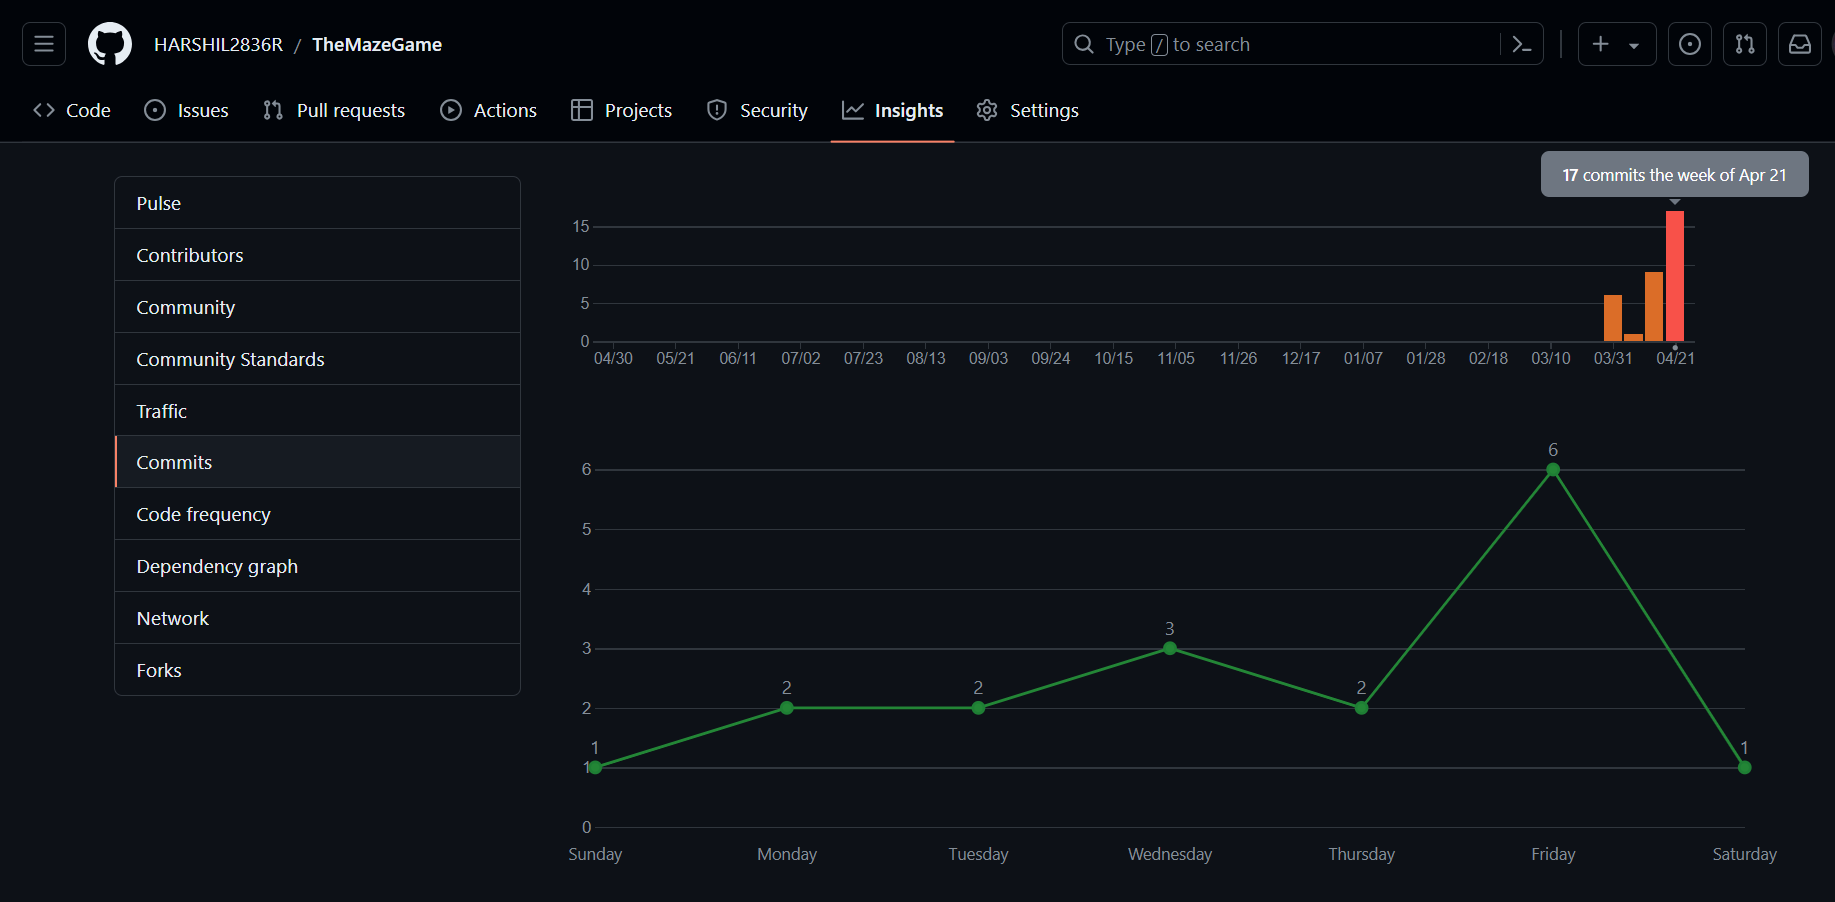
\includegraphics[width=\textwidth]{screenshots/commits.png}
        \caption[(a)]{Commit history in git}
        \label{fig:commit}
    \end{subfigure}
    \begin{subfigure}[b]{0.5\textwidth}
        \centering
        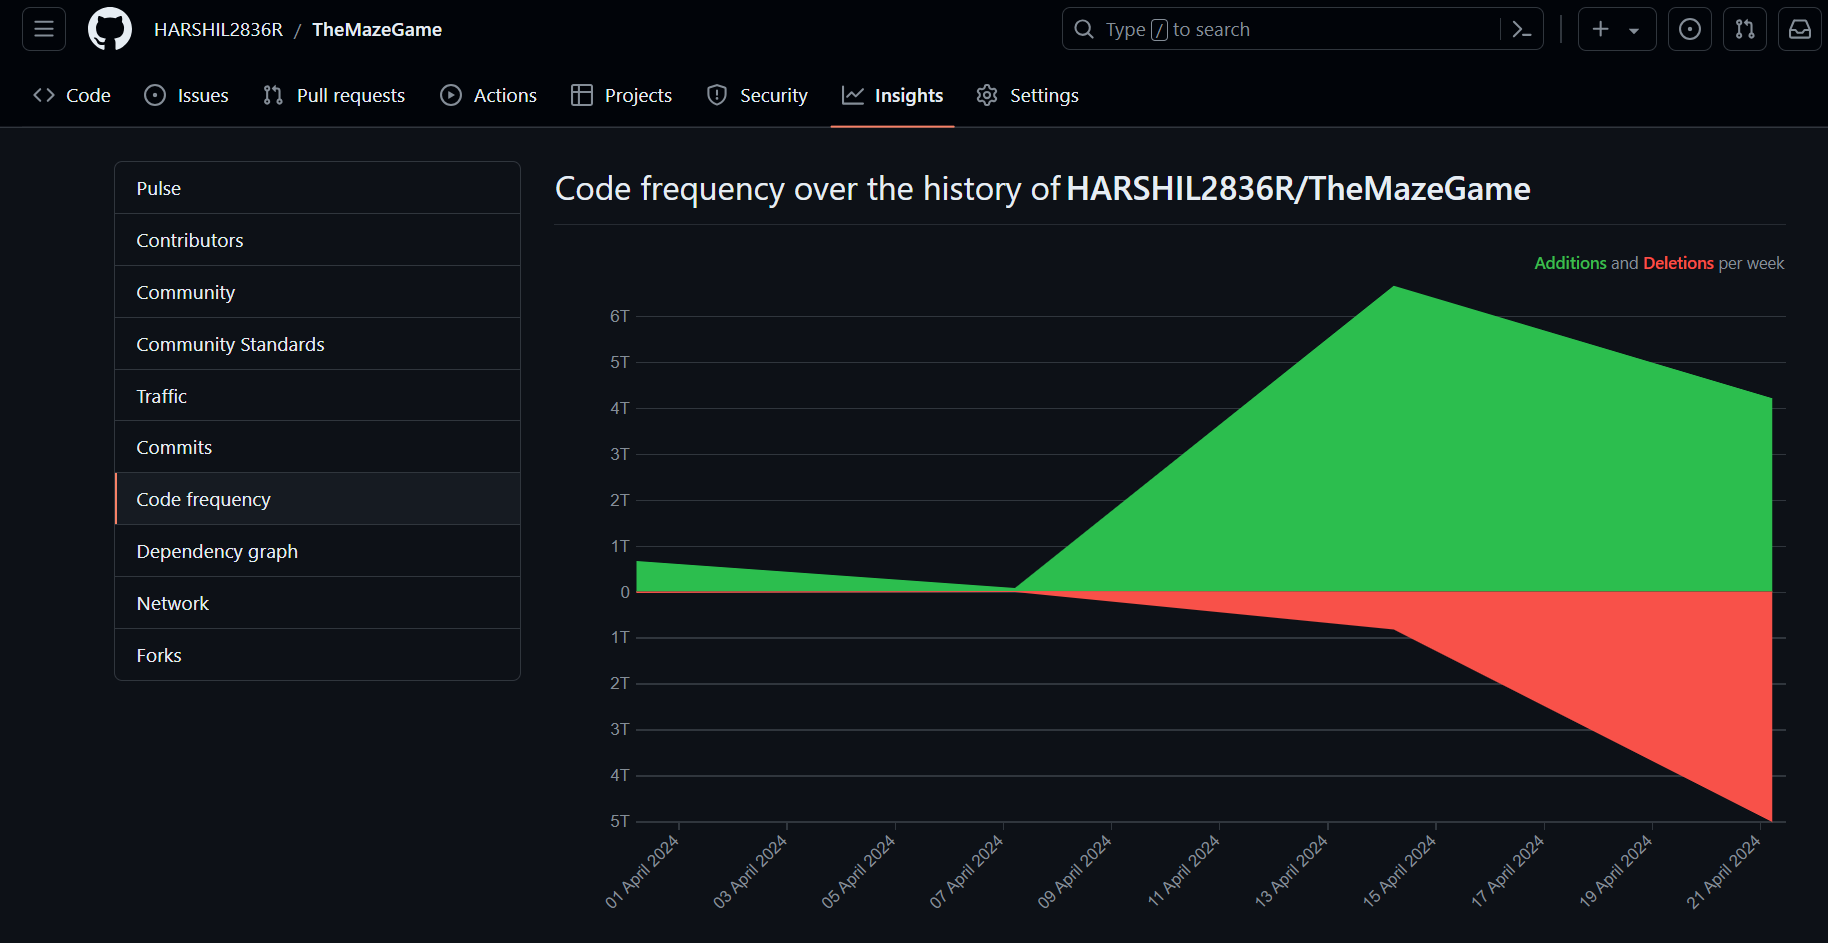
\includegraphics[width=\textwidth]{screenshots/code_freq.png}
        \caption[(a)]{Code frequency over history in git}
        \label{fig:code_freq}
    \end{subfigure}
\end{figure}

\subsection{The Book}
I started my project by solely refering to the book \textit{Python Crash Course}~\cite*{thebook} provided as a reference by the TA. It gave the fundamental basis to my game and showed me the power of Classes in building big projects. I created the Settings class and Player class.\\
Then I implemented the menu in the game, learning first time about pygame Rects and Surfaces and how to blit them as Interactive buttons~\cite{menu-geeksforgeeks} and~\cite{rendering_text}. Created the Buttons class. I also stared write notes in file \texttt{README.md}\cite{md-reference}.\\
\subsection{The Maze matrix}
After making the menu I started to Research over the different Maze generation algorithms available. I came across \href{https://stackoverflow.com/questions/38502/whats-a-good-algorithm-to-generate-a-maze}{this answer} on StackExchange~\cite*{stack-exchange-algorithms} and have added the Algorithms I studied in Maze Generation Algorithms section (Section~\ref{maze_algs}). I wasted a few hours figuring out how to start the walk but my code didn't work. Next day I started with a sample code from replit~\cite*{replit} and based on it built my random walk fine-tuning it and adding additional parameters such as the range of steps the walk should consist of. Here are the Screenshots of my working out the random walk, Fig.~\ref{fig:20x20random_walk} and Fig.~\ref{fig:40x40random_walk}\\

\begin{figure}[h]
    \caption[1]{}
    \begin{subfigure}[b]{0.5\textwidth}
        \centering
        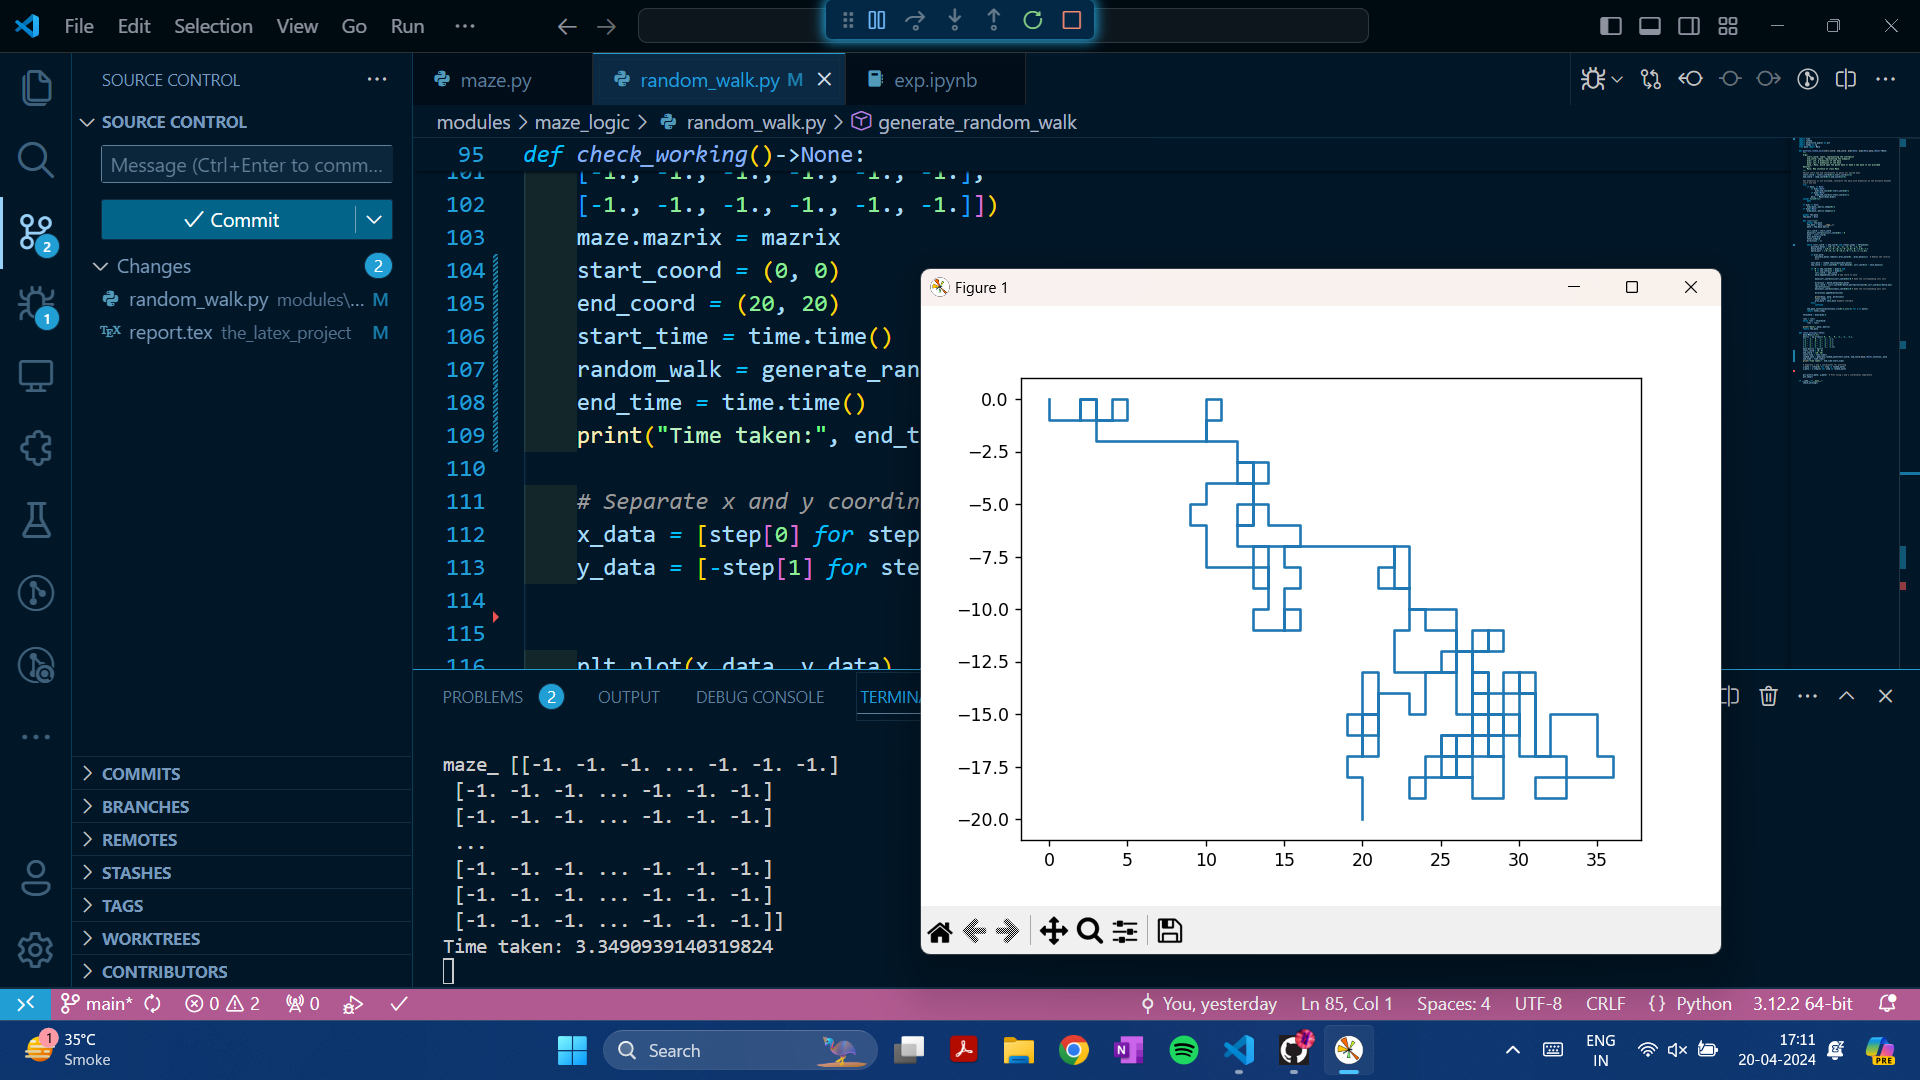
\includegraphics[width=\textwidth]{screenshots/Screenshot (164).png}
        \caption[(a)]{20x20 random walk without grid constraint}
        \label{fig:20x20random_walk}
    \end{subfigure}
    \begin{subfigure}[b]{0.5\textwidth}
        \centering
        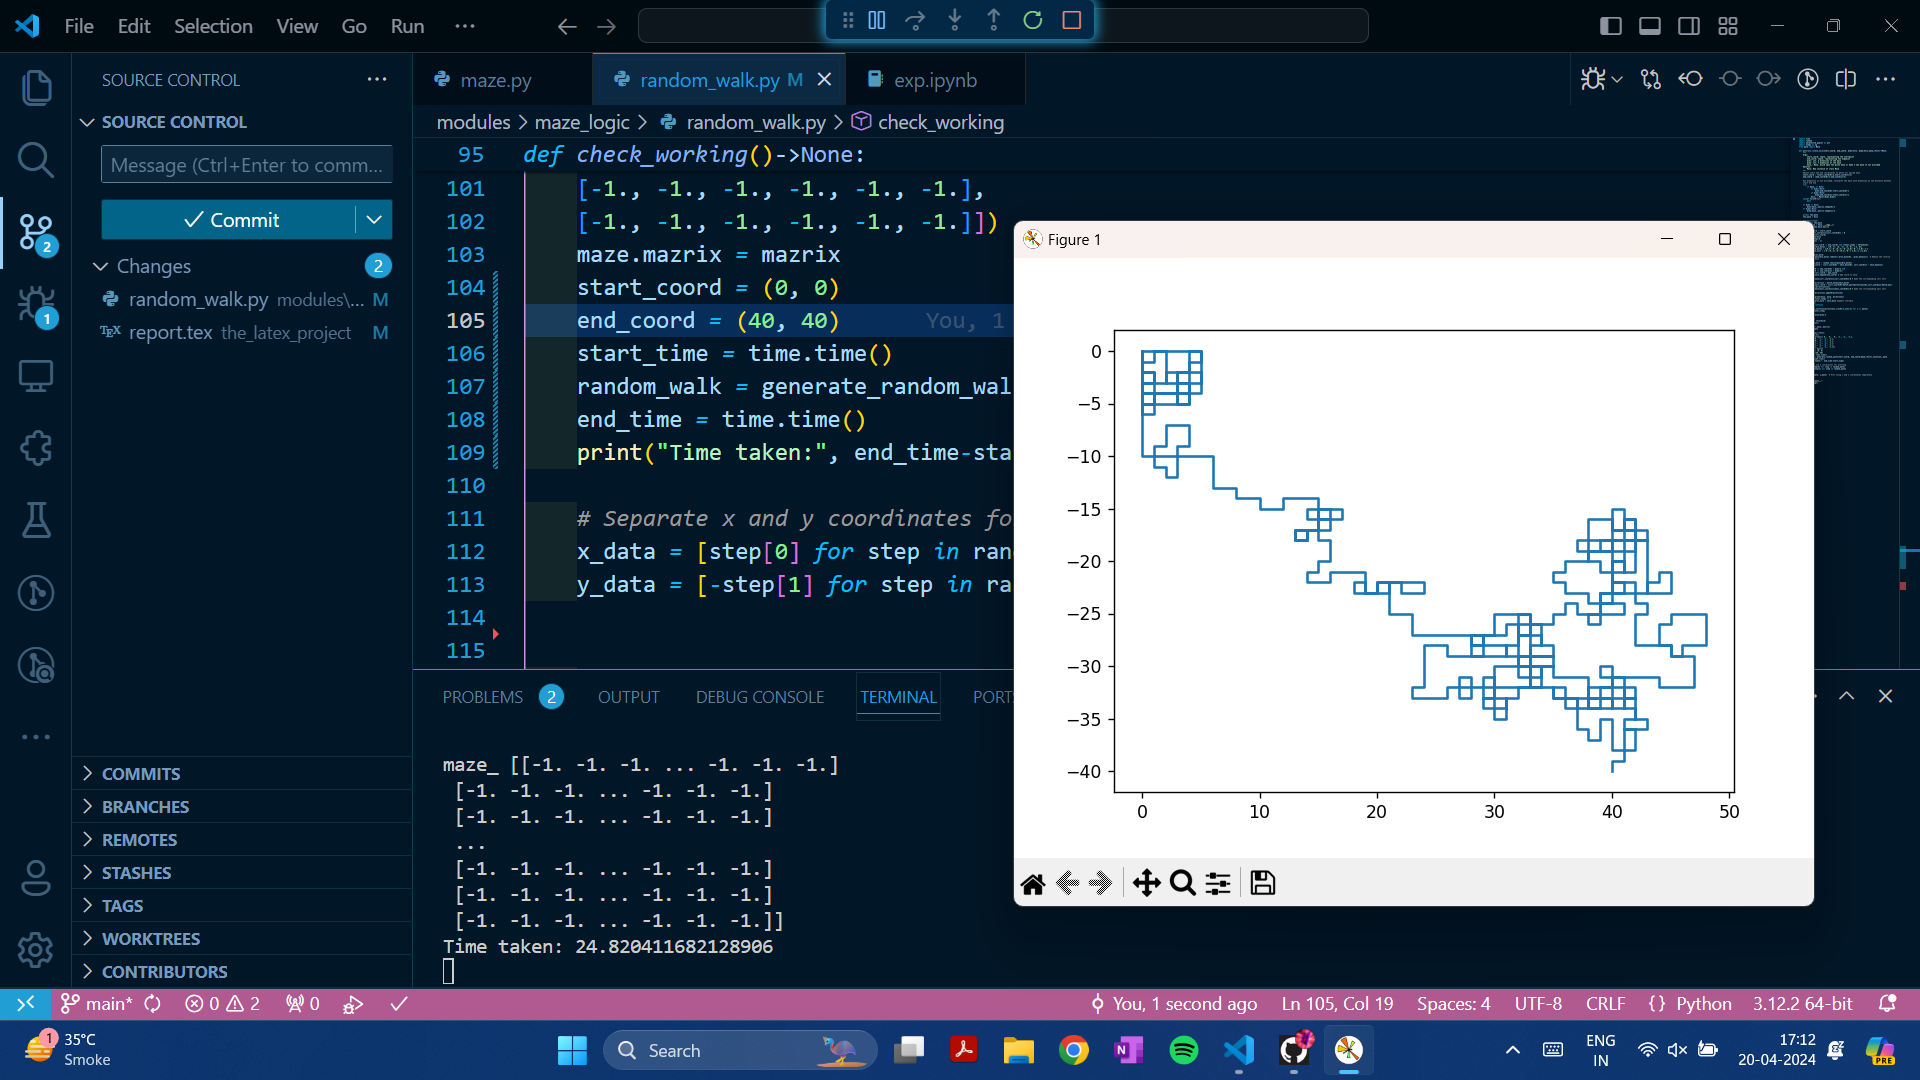
\includegraphics[width=\textwidth]{screenshots/Screenshot (166).png}
        \caption[(a)]{40x40 random walk without grid constraint}
        \label{fig:40x40random_walk}
    \end{subfigure}
\end{figure}

Getting Inspiration from all these Algorithms and understanding how randomness is used in each algorithm, I created my own Algorithm here~\ref{my_alg}
Then I made the game dynamic by allowing the player to move and deploying the camera (while keeping the complete map layout as it is, so it can also be accessed by tweaking the code in settings)
\subsection{The Map}
Before the Camera class was created I was blitting object directly to the screen as a map, here are screenshots of that, Fig.~\ref{fig:map1} and Fig.~\ref{fig:map2}
\begin{figure}[h]
    \caption[1]{}
    \begin{subfigure}[b]{0.5\textwidth}
        \centering
        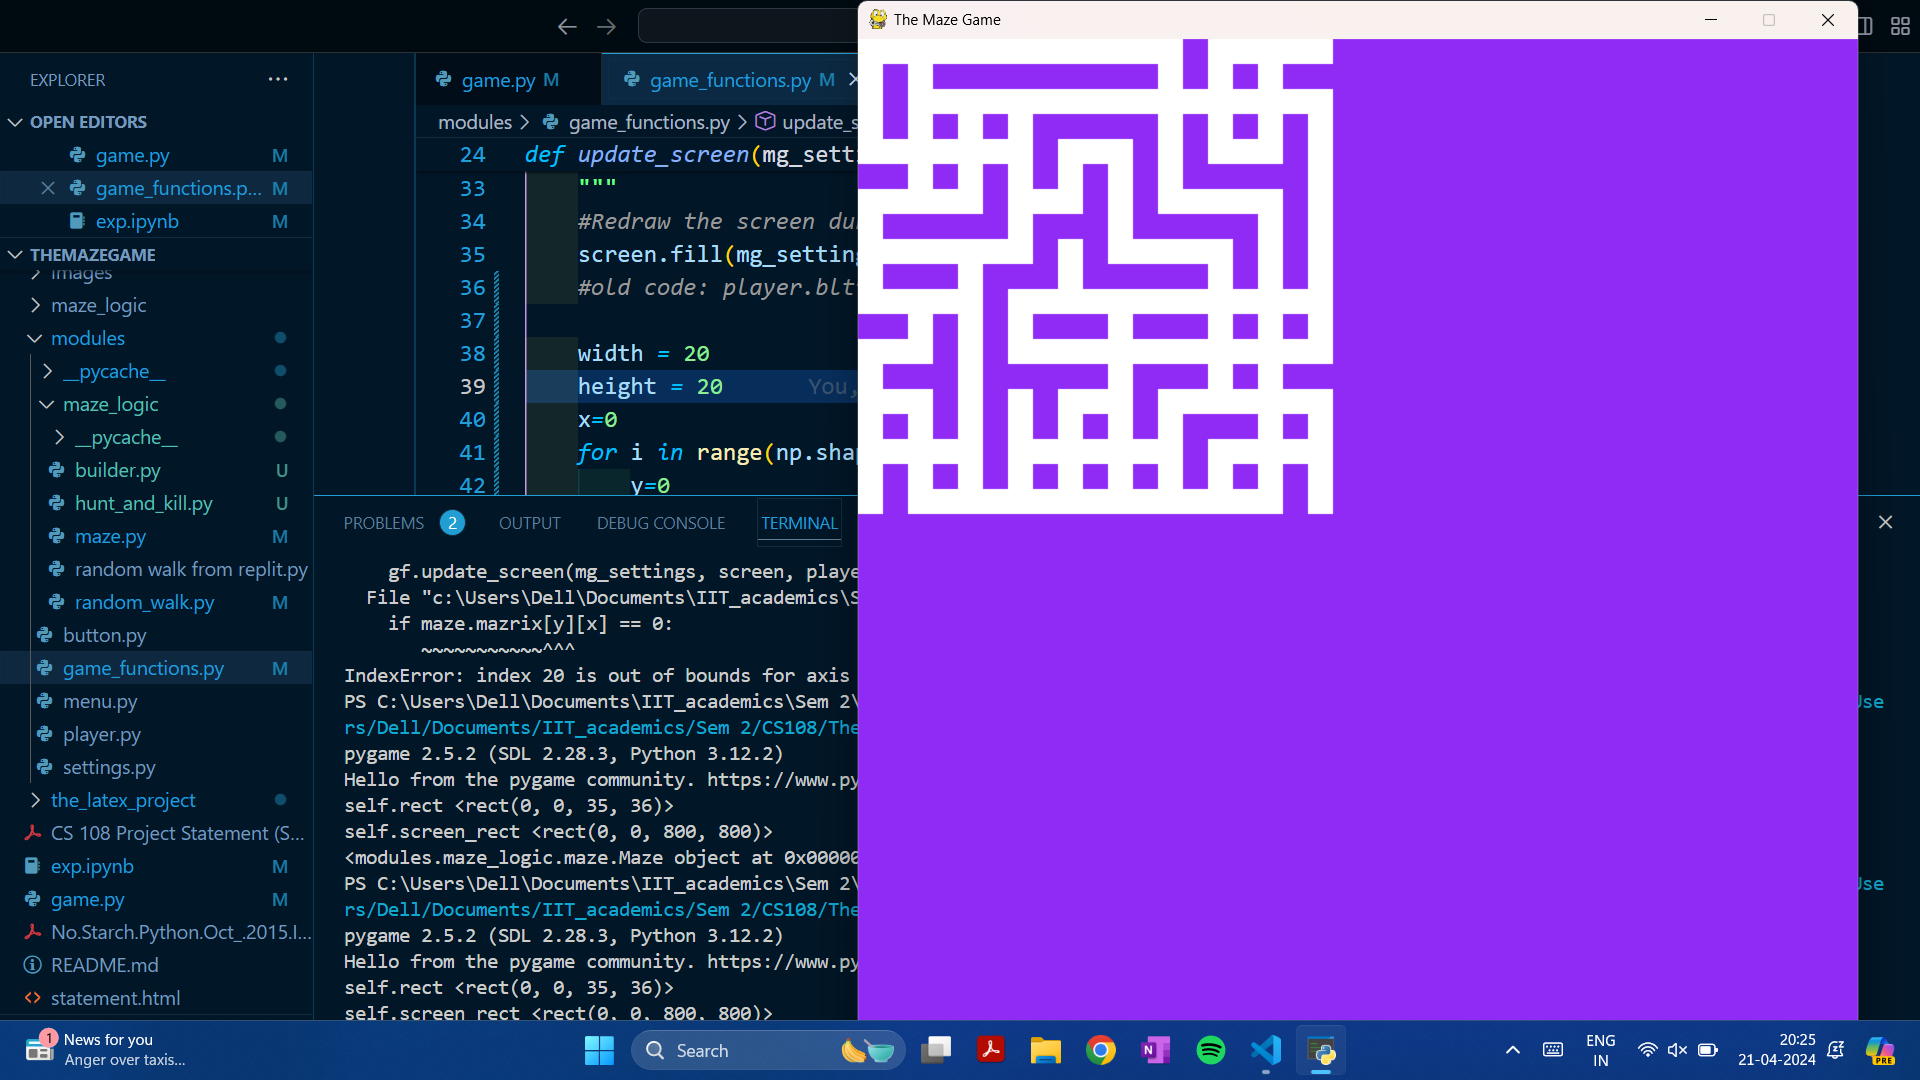
\includegraphics[width=\textwidth]{screenshots/Screenshot (168).png}
        \caption[(a)]{First Maze I blitted into pygame screen}
        \label{fig:map1}
    \end{subfigure}
    \begin{subfigure}[b]{0.5\textwidth}
        \centering
        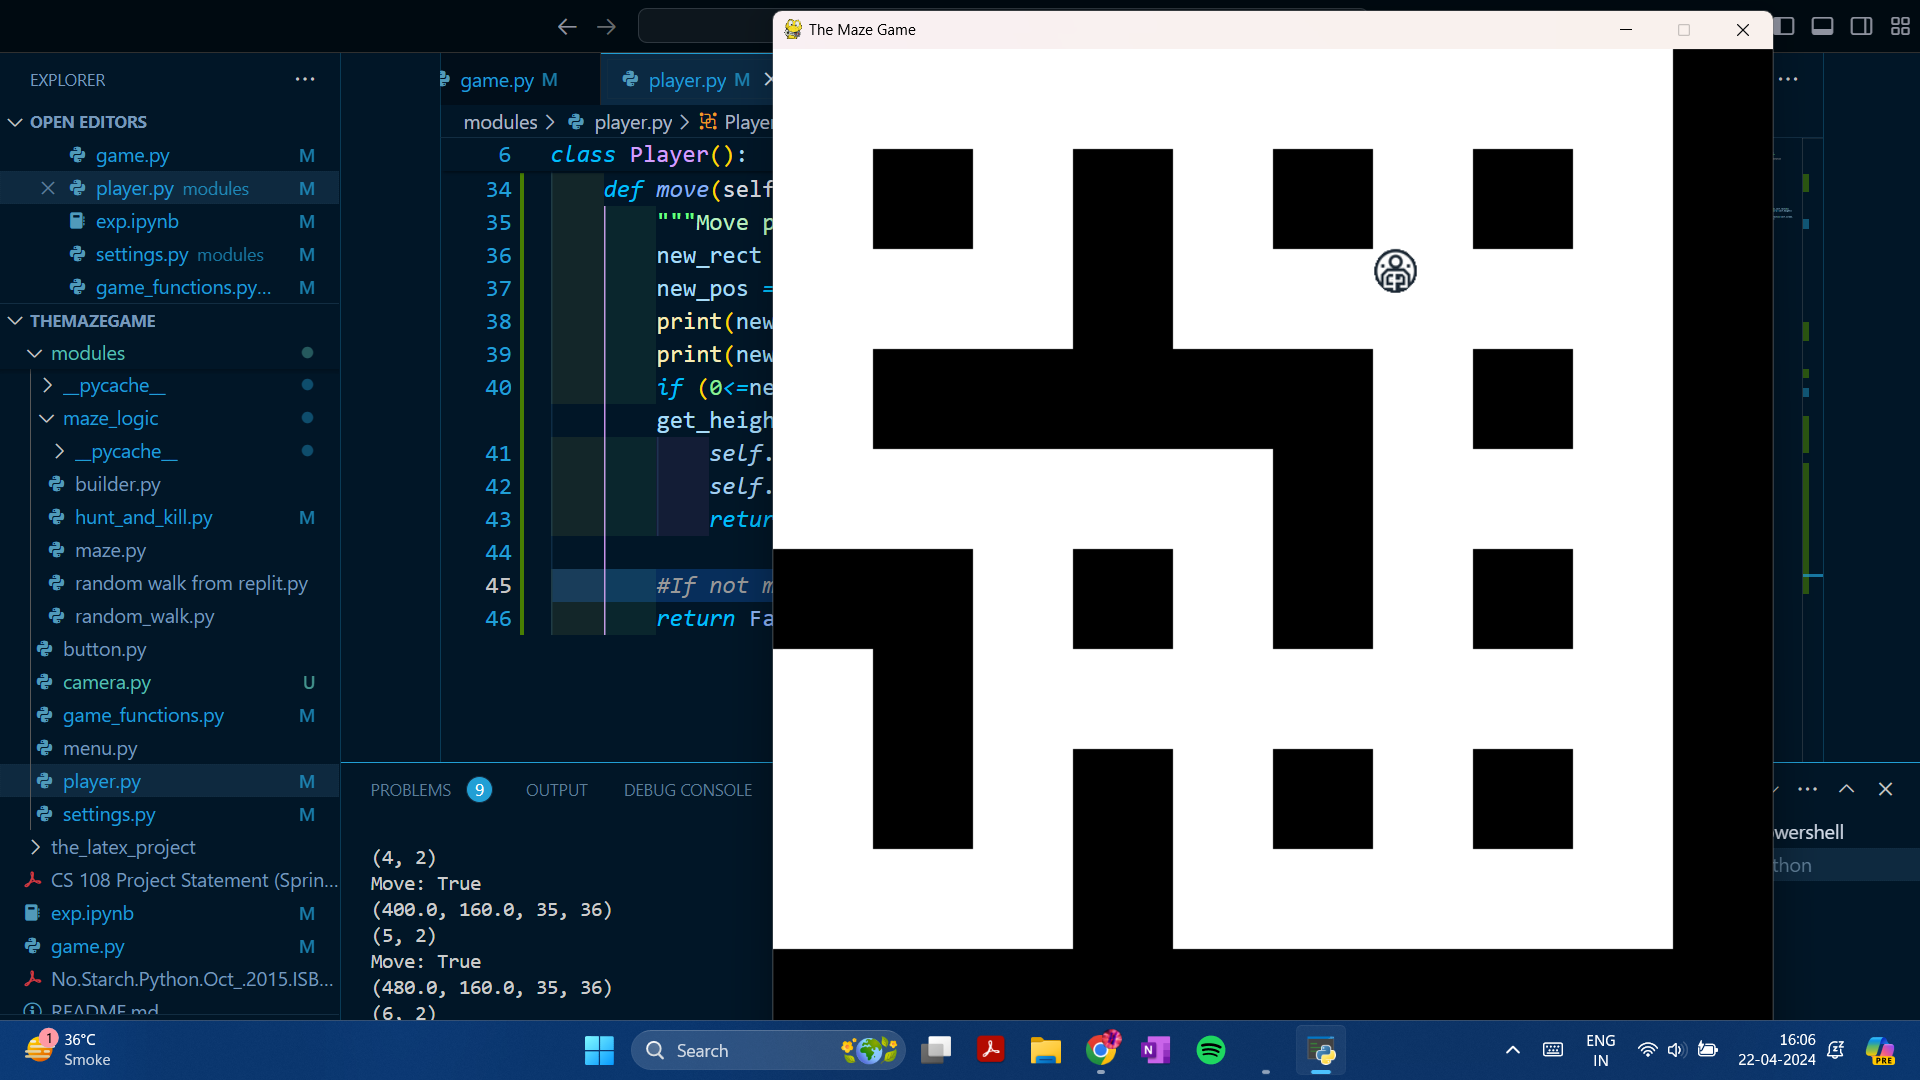
\includegraphics[width=\textwidth]{screenshots/Screenshot (169).png}
        \caption[(a)]{Scaled the maze to match screen size and blit player}
        \label{fig:map2}
    \end{subfigure}
\end{figure}

Final map view looked like this, Fig.~\ref{fig:map3}, Fig.~\ref{fig:map4} and Fig.~\ref{fig:map5}

\begin{figure}[h]
    \caption[1]{}
    \centering
    \begin{subfigure}[b]{0.4\textwidth}
        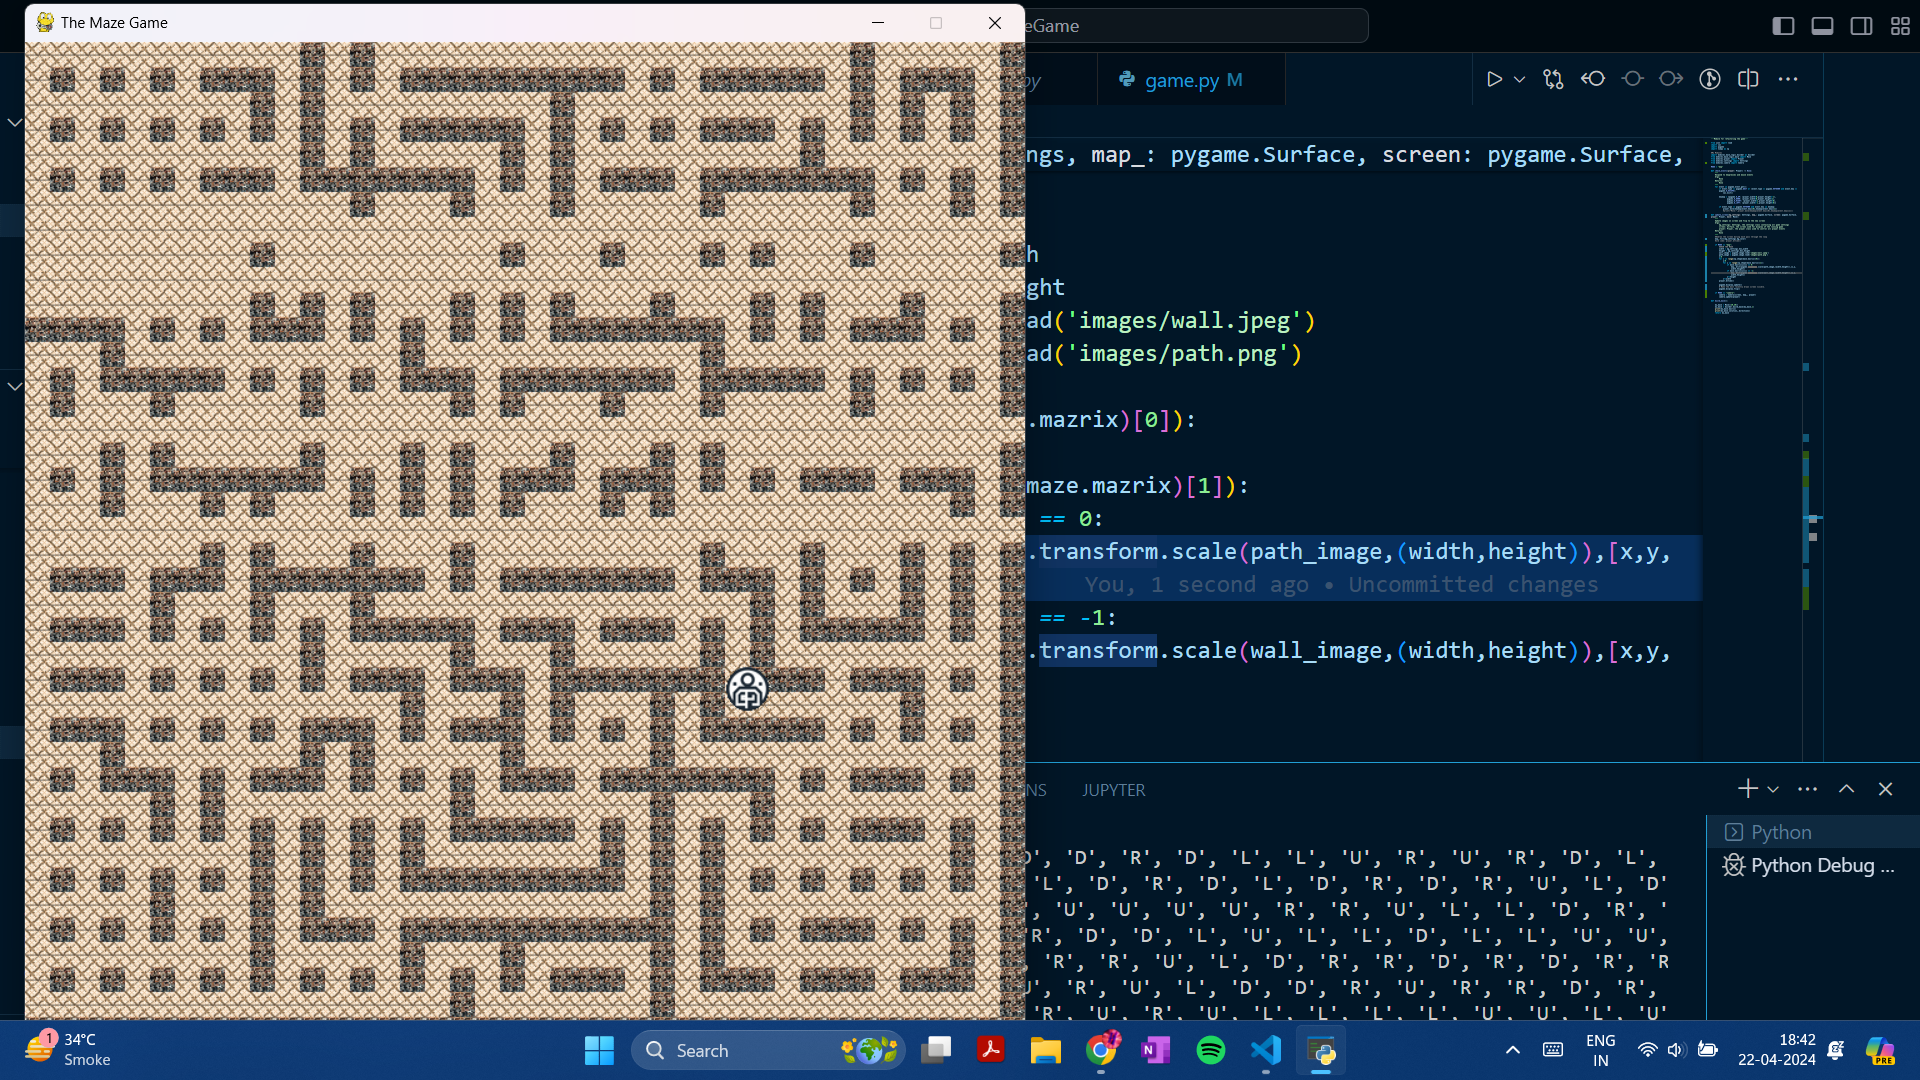
\includegraphics[width=\textwidth]{screenshots/Screenshot (170).png}
        \caption[(a)]{20x20 Maze}
        \label{fig:map3}
    \end{subfigure}
    \hfil
    \begin{subfigure}[b]{0.4\textwidth}
        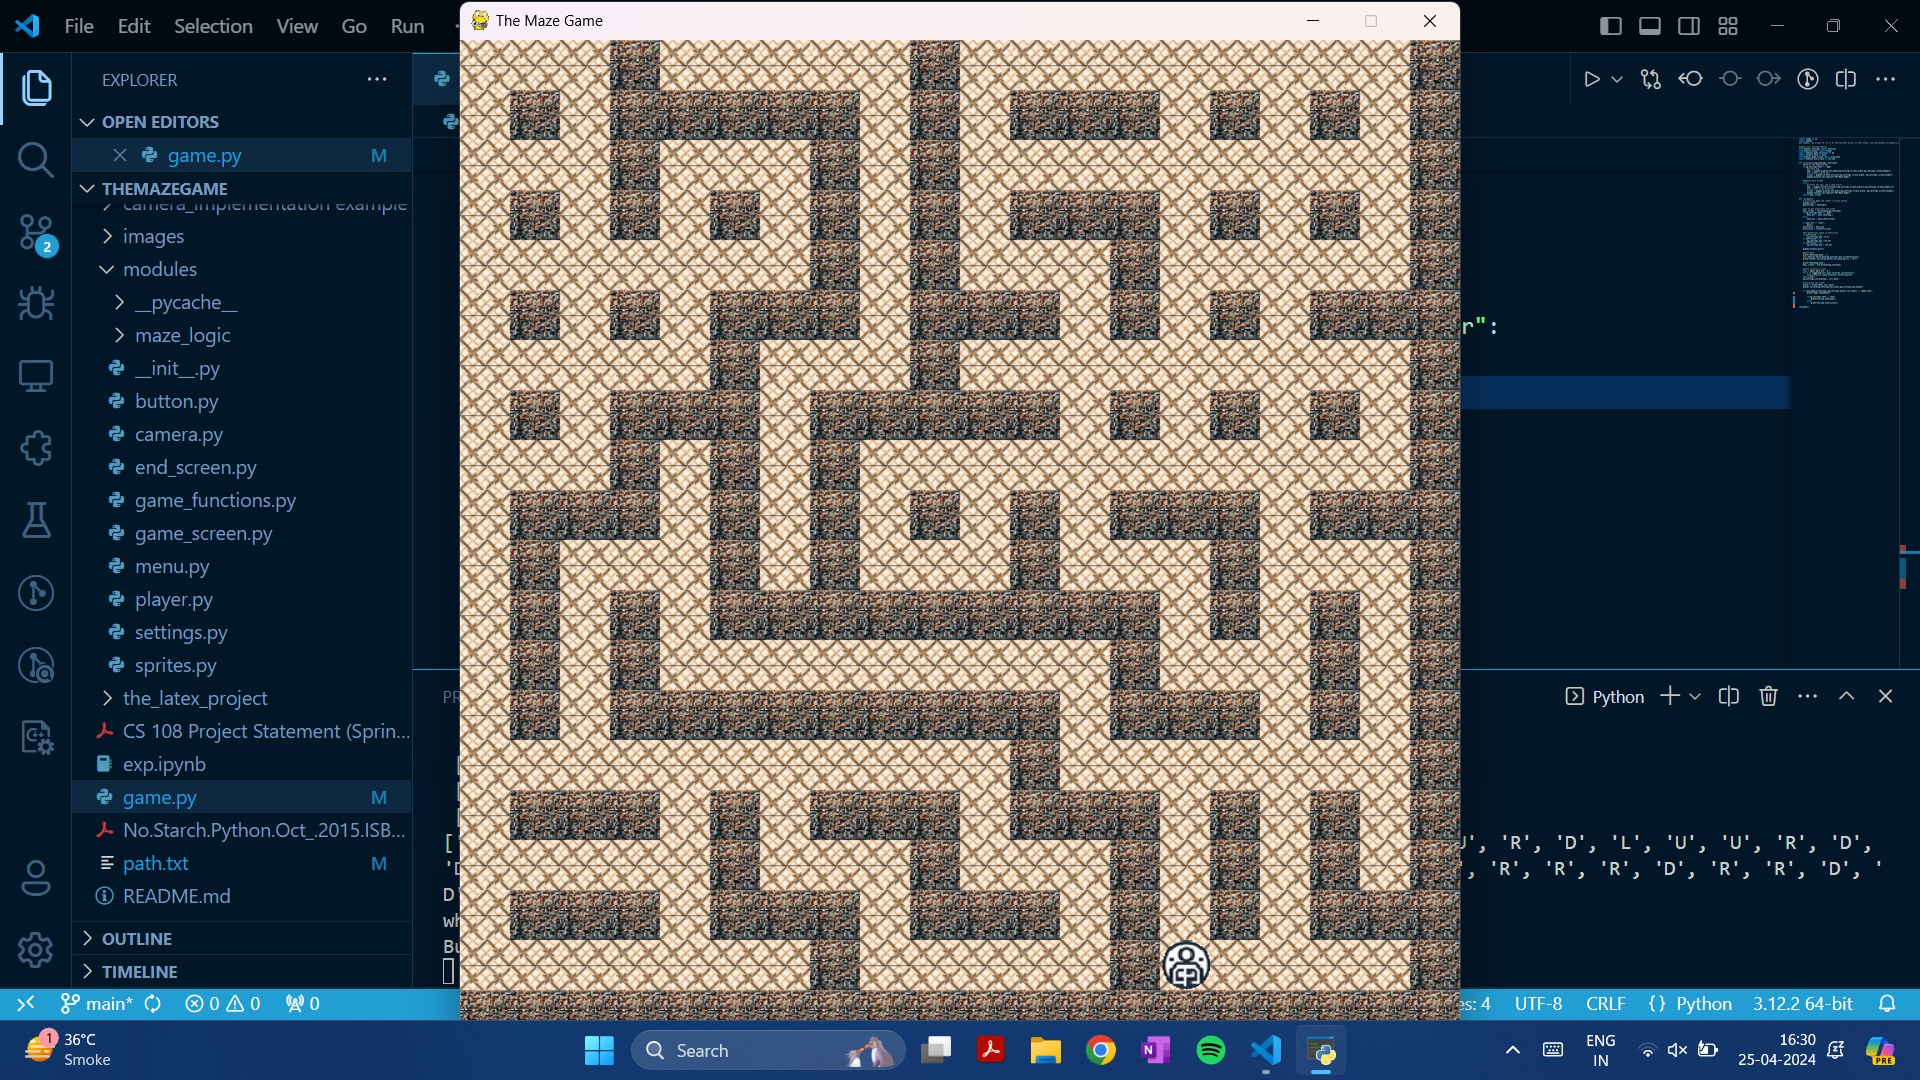
\includegraphics[width=\textwidth]{screenshots/Screenshot (172).png}
        \caption[(a)]{10x10 Maze}
        \label{fig:map4}
    \end{subfigure}
    \begin{subfigure}[r]{0.5\textwidth}
        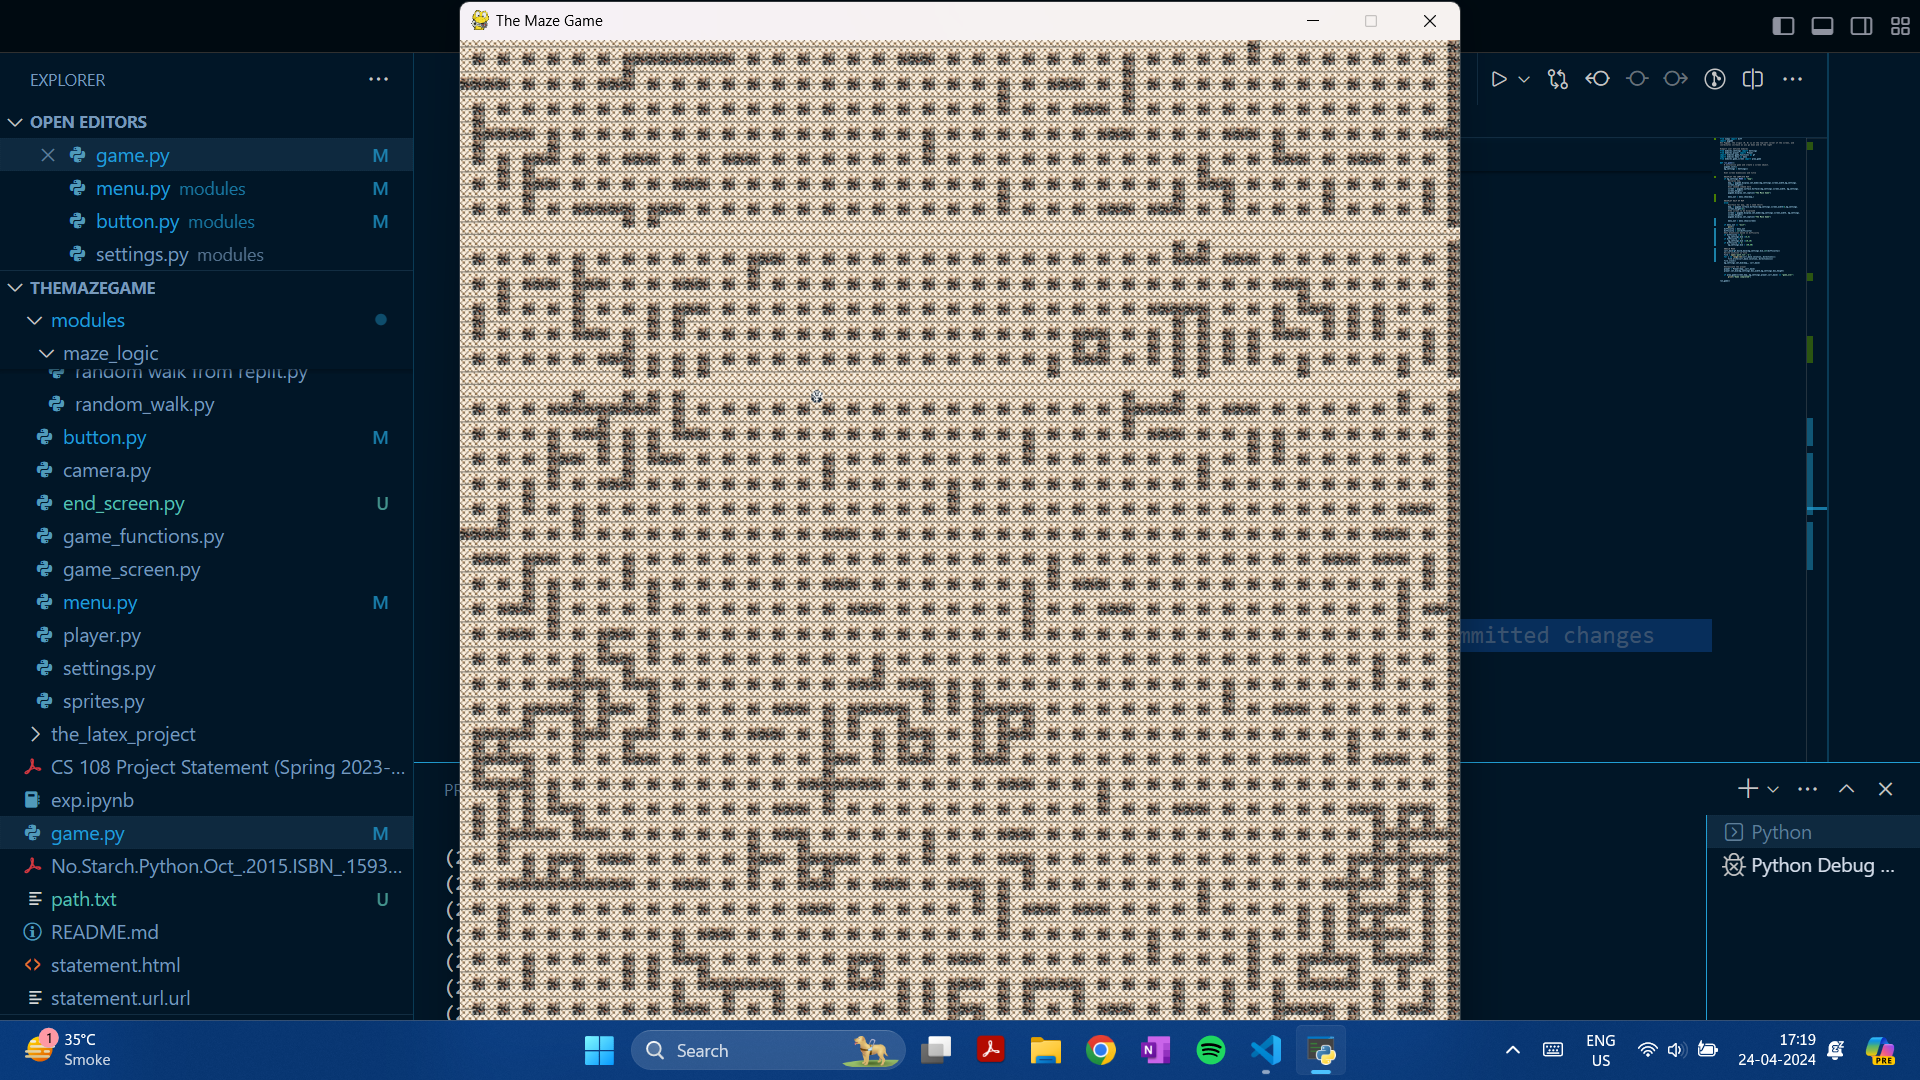
\includegraphics[width=\textwidth]{screenshots/Screenshot (171).png}
        \caption[(a)]{40x40 Maze}
        \label{fig:map5}
    \end{subfigure}
\end{figure}

\subsection{The Camera and The Pegion}
For the Camera to function efficiently~\cite{camera_tutorial}, I needed the \textit{"things"}, i.e. the player and wall and path Rects to be Sprites (children of class pygame.sprite.Sprite) hence I redefined the classes a bit and learnt more about Sprites and Groups in pygame~\cite{sprite_reference}. I also used groups to create animation effect in End-Screen~\cite*{end-scren_animation}. After implementing the camera, the game looked like, Fig.~\ref{fig:camera1} and end-screen like Fig.~\ref{fig:camera2}.

\begin{figure}[h]
    \caption[1]{}
    \begin{subfigure}[b]{0.5\textwidth}
        \centering
        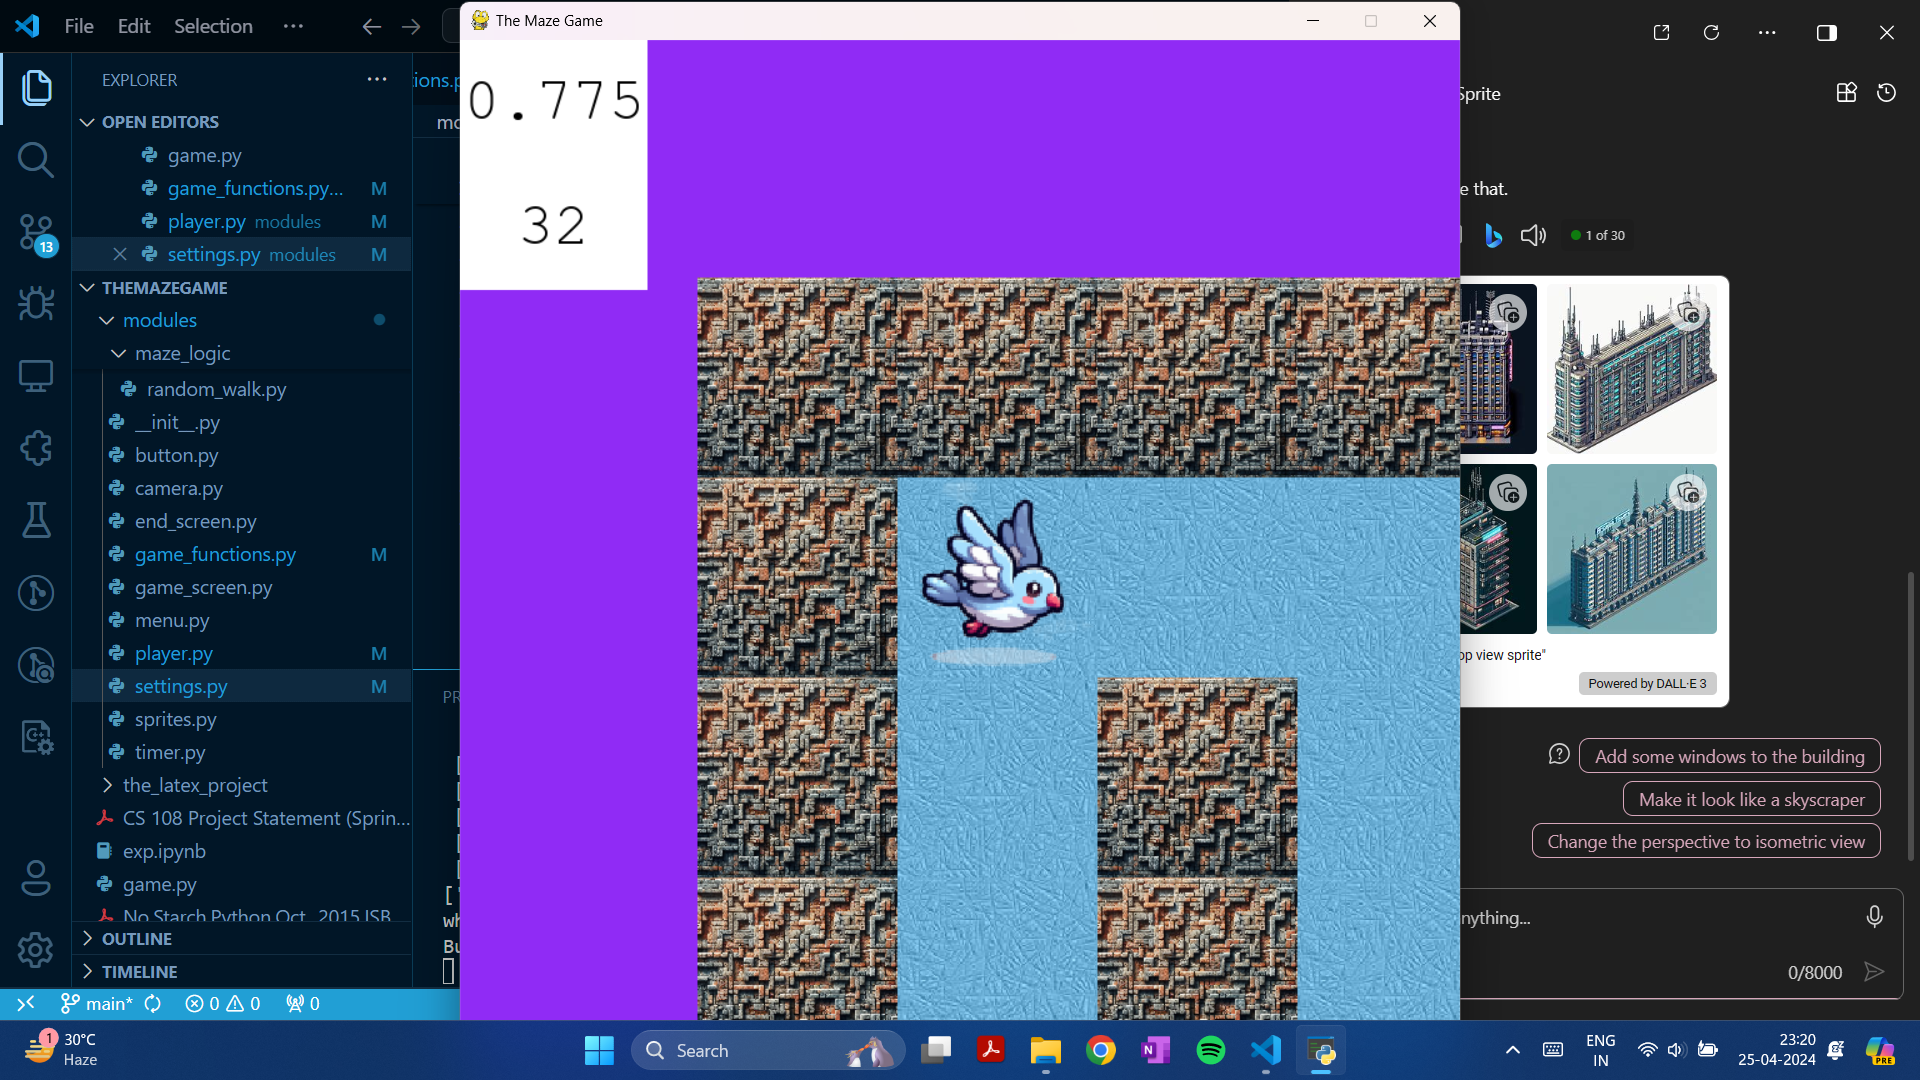
\includegraphics[width=\textwidth]{screenshots/Screenshot (174).png}
        \caption[(a)]{Starting Camera screen where pegion is deployed}
        \label{fig:camera1}
    \end{subfigure}
    \begin{subfigure}[b]{0.5\textwidth}
        \centering
        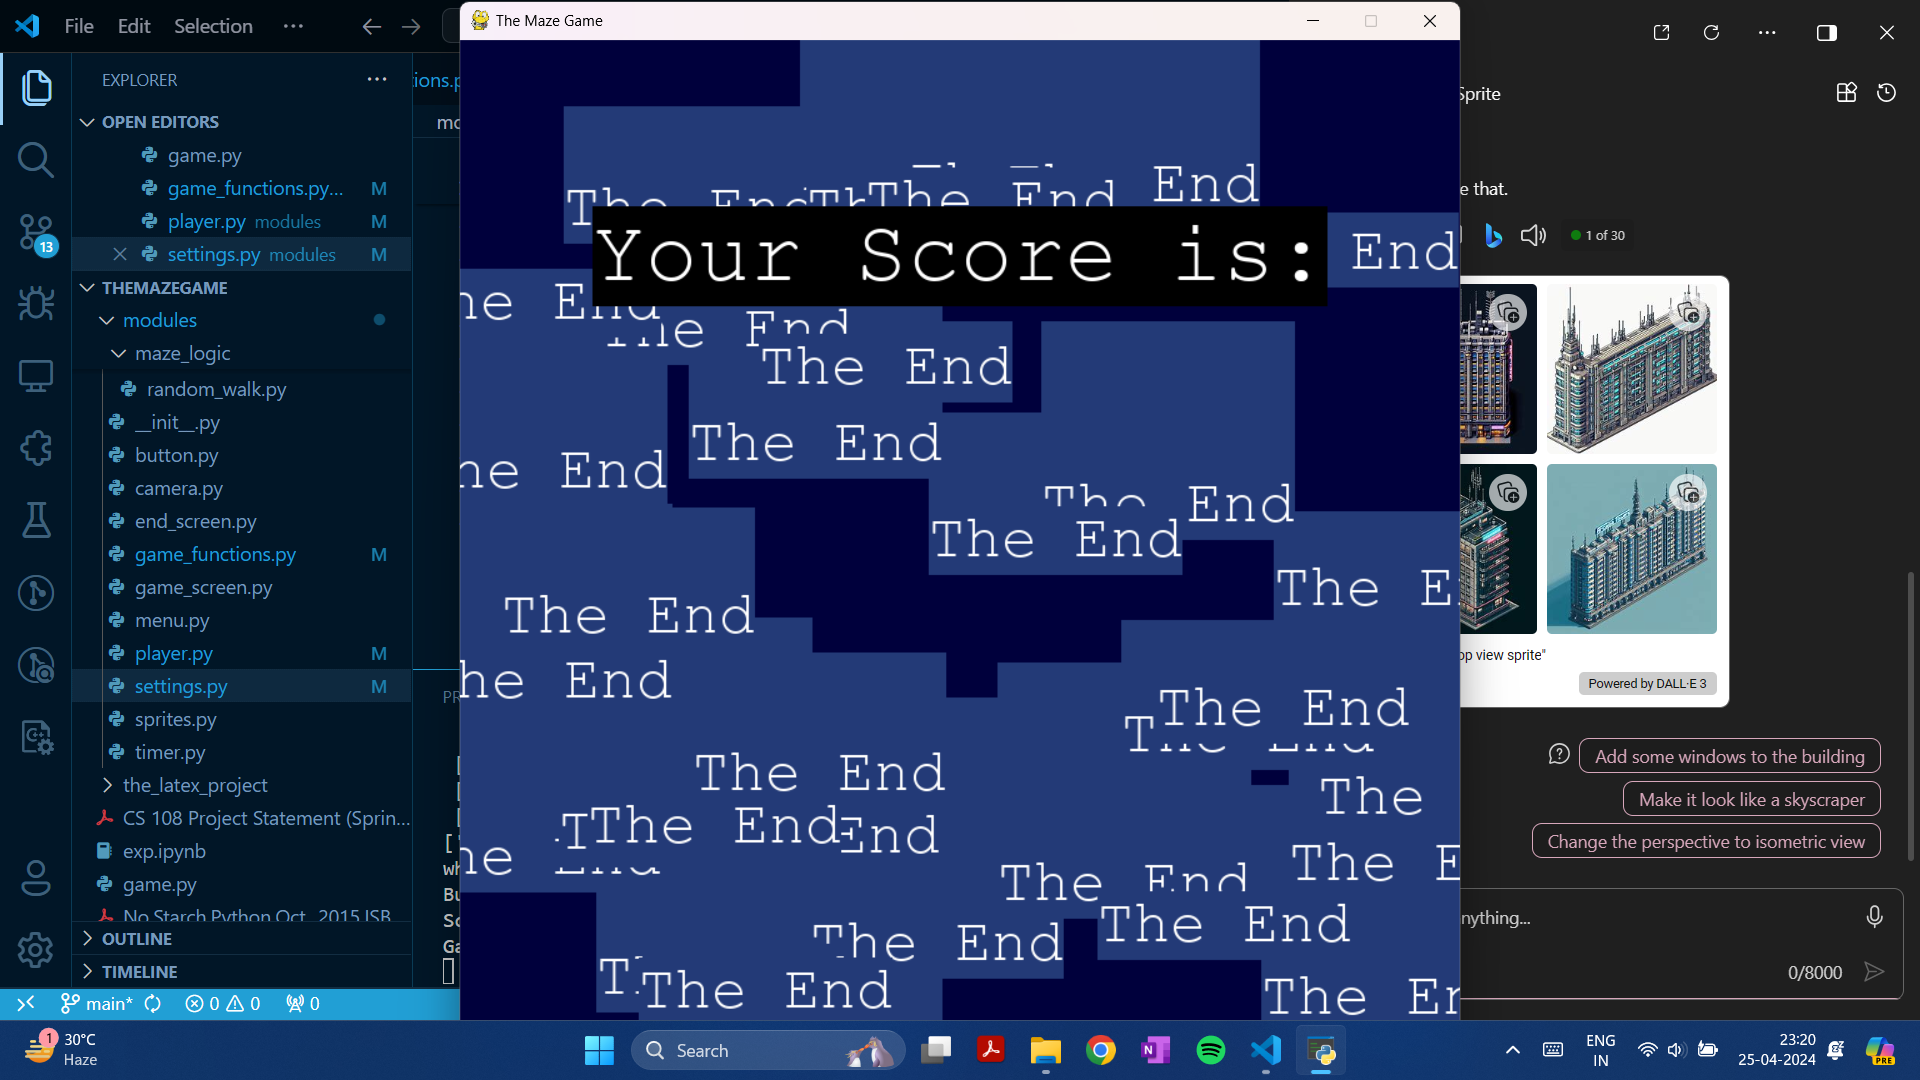
\includegraphics[width=\textwidth]{screenshots/Screenshot (175).png}
        \caption[(a)]{Animated End-Screen, incomplete}
        \label{fig:camera2}
    \end{subfigure}
\end{figure}



\subsection{Git Log}
Here's the output of command \texttt{git log --graph --oneline --stat --color} with changes to .pyc files and changes to the another Game project~\cite*{camera_reference} I referred to for building up camera in my game, removed.

%%%%% WRITING git log --graph --oneline --color OUTPUT TO Document 
{
\let\XXegroup\relax
\expandafter\def\csname XX[31\endcsname{%
    \bgroup\let\XXegroup\egroup\leavevmode\color{red}}
\expandafter\def\csname XX[1;31\endcsname{%
    \bgroup\let\XXegroup\egroup\leavevmode\bfseries\color{red}}
\expandafter\def\csname XX[32\endcsname{%
    \bgroup\let\XXegroup\egroup\leavevmode\color{green}}
\expandafter\def\csname XX[1;32\endcsname{%
    \bgroup\let\XXegroup\egroup\leavevmode\bfseries\color{green}}
\expandafter\def\csname XX[33\endcsname{%
    \bgroup\let\XXegroup\egroup\leavevmode\color{yellow}}
\expandafter\def\csname XX[1;33\endcsname{%
    \bgroup\let\XXegroup\egroup\leavevmode\bfseries\color{yellow}}
\expandafter\def\csname XX[34\endcsname{%
    \bgroup\let\XXegroup\egroup\leavevmode\color{cyan}}
\expandafter\def\csname XX[1;34\endcsname{%
    \bgroup\let\XXegroup\egroup\leavevmode\bfseries\color{cyan}}
\expandafter\def\csname XX[35\endcsname{%
    \bgroup\let\XXegroup\egroup\leavevmode\color{magenta}}
\expandafter\def\csname XX[1;35\endcsname{%
    \bgroup\let\XXegroup\egroup\leavevmode\bfseries\color{magenta}}
\expandafter\def\csname XX[36\endcsname{%
    \bgroup\let\XXegroup\egroup\leavevmode\color{blue}}
\expandafter\def\csname XX[1;36\endcsname{%
    \bgroup\let\XXegroup\egroup\leavevmode\bfseries\color{blue}}


\expandafter\def\csname XX[\endcsname{\XXegroup}
\catcode`\^^[=13
\def^^[#1m{%
\expandafter\ifx\csname XX#1\endcsname\relax
\typeout{XX#1}%
\else
\csname XX#1\endcsname
\fi}
\

\begin{verbatim}
    * 8c85451 remove unwanted things, update problem statement, work on report
    |  ...Spring 2023-24) _ Maze Game in Python.pdf |  Bin 3332129 -> 3343895 bytes
    |  data/saved_data.csv                          |   12 +-
    |  exp.ipynb                                    |    3 -
    |  last_maze.txt                                |   20 +
    |  modules/button.py                            |   25 +-
    |  modules/camera.py                            |   27 +-
    |  modules/end_screen.py                        |   19 +-
    |  modules/game_functions.py                    |   14 +-
    |  modules/maze_logic/builder.py                |    6 +-
    |  modules/maze_logic/hunt_and_kill.py          |   22 +-
    |  modules/maze_logic/maze.py                   |   54 +-
    |  .../maze_logic/random walk from replit.py    |   36 -
    |  modules/maze_logic/random_walk.py            |   41 +-
    |  modules/menu.py                              |    3 +-
    |  modules/settings.py                          |   10 +-
    |  modules/sprites.py                           |    4 +
    |  modules/timer.py                             |   25 +-
    |  notes.md                                     |   24 +-
    |  path.txt                                     |    2 +-
    |  the_latex_project/report.aux                 |   25 +-
    |  the_latex_project/report.bcf-SAVE-ERROR      | 2364 ----------------
    |  the_latex_project/report.blg                 |   17 -
    |  the_latex_project/report.fdb_latexmk         |   32 +-
    |  the_latex_project/report.fls                 |   44 +-
    |  the_latex_project/report.log                 |  202 +-
    |  the_latex_project/report.out                 |   23 +-
    |  the_latex_project/report.pdf                 |  Bin 136846 -> 187644 bytes
    |  the_latex_project/report.synctex.gz          |  Bin 28646 -> 53120 bytes
    |  the_latex_project/report.tex                 |   98 +-
    |  the_latex_project/report.toc                 |   23 +-
    |  107 files changed, 528 insertions(+), 4344 deletions(-)
    * ddcff22 rename readme
    |  README.md => notes.md | 0
    |  1 file changed, 0 insertions(+), 0 deletions(-)
    * 5de56d0 organise and comment things
    |  README.md                                    |  59 ++++++++++++-
    |  data/saved_data.csv                          |   5 +-
    |  game.py                                      |  32 ++++++-
    |  images/player.png                            | Bin 3002 -> 12946 bytes
    |  images/player3.png                           | Bin 12946 -> 0 bytes
    |  images/player_old.png                        | Bin 0 -> 3002 bytes
    |  modules/game_functions.py                    |   3 +-
    |  modules/game_screen.py                       |  11 +++
    |  modules/player.py                            |  27 ++++--
    |  modules/settings.py                          |  75 +++++++++++++----
    |  path.txt                                     |   2 +-
    |  the_latex_project/references.bib             |   2 +-
    |  the_latex_project/report.aux                 |   5 +-
    |  the_latex_project/report.bbl                 |  13 +++
    |  the_latex_project/report.bcf                 |   1 +
    |  the_latex_project/report.blg                 |  28 +++---
    |  the_latex_project/report.fdb_latexmk         |  27 +++---
    |  the_latex_project/report.fls                 |   6 ++
    |  the_latex_project/report.log                 |  28 +++---
    |  the_latex_project/report.pdf                 | Bin 112827 -> 136846 bytes
    |  the_latex_project/report.synctex.gz          | Bin 28106 -> 28646 bytes
    |  the_latex_project/report.tex                 |  11 +++
    |  26 files changed, 270 insertions(+), 65 deletions(-)
    * cce1681 Improve references.bib
    |  ...toy-sound.mp3 => duck-toy-sound_copy.mp3} | Bin
    |  audio/ducky-toy-sound.mp3                    | Bin 0 -> 17059 bytes
    |  audio/ducky-toy-sound.mp4                    | Bin 0 -> 24907 bytes
    |  data/saved_data.csv                          |   5 +-
    |  modules/game_functions.py                    |   2 +-
    |  modules/game_screen.py                       |   4 +-
    |  path.txt                                     |   2 +-
    |  the_latex_project/references.bib             |  96 ++++-------------
    |  10 files changed, 28 insertions(+), 81 deletions(-)
    * 80cff37 basic requirements fulfilled
    |  .../angry-birds-theme-song-audiotrimmer.mp3  | Bin 0 -> 129913 bytes
    |  ...ter-strike-jingle-cs-radio-ok-lets-go.mp3 | Bin 0 -> 26677 bytes
    |  audio/duck-toy-sound.mp3                     | Bin 0 -> 30765 bytes
    |  audio/gta-v-death-sound-effect-102.mp3       | Bin 0 -> 124804 bytes
    |  audio/happy-happy-happy-song.mp3             | Bin 0 -> 303291 bytes
    |  .../punch-gaming-sound-effect-hd_RzlG1GE.mp3 | Bin 0 -> 25423 bytes
    |  audio/super-mario-beedoo_F3cwLoe.mp3         | Bin 0 -> 133870 bytes
    |  data/saved_data.csv                          |  28 ++++++++++++++-
    |  game.py                                      |  32 +++++++++++++----
    |  modules/end_screen.py                        |  19 +++++++---
    |  modules/game_functions.py                    |  19 +++++-----
    |  modules/game_screen.py                       |   2 +-
    |  path.txt                                     |   2 +-
    |  the_latex_project/references.bib             |  10 ++++++
    |  19 files changed, 89 insertions(+), 23 deletions(-)
    * f475a3f Complete End Screen and start adding sound
    |  audio/caproni.mp3                            | Bin 0 -> 4276122 bytes
    |  audio/wind.wav                               | Bin 0 -> 1059244 bytes
    |  data/saved_data.csv                          |  76 ++++++-----------
    |  game.py                                      |   5 +-
    |  images/nest.png                              | Bin 0 -> 426146 bytes
    |  images/nest2.png                             | Bin 0 -> 578484 bytes
    |  modules/camera.py                            |   1 +
    |  modules/end_screen.py                        |  28 ++++++
    |  modules/game_functions.py                    |  16 +++-
    |  modules/game_screen.py                       |  15 +++-
    |  modules/maze_logic/builder.py                |  15 ++--
    |  modules/maze_logic/hunt_and_kill.py          |   7 ++
    |  modules/maze_logic/random_walk.py            |   2 +-
    |  modules/player.py                            |   3 +-
    |  modules/settings.py                          |  18 +++-
    |  modules/timer.py                             |   3 +-
    |  path.txt                                     |   2 +-
    |  27 files changed, 119 insertions(+), 72 deletions(-)
    * 70ec88f improve sprites
    |  data/saved_data.csv                          |  40 +++++++++++++++++
    |  game.py                                      |   2 +
    |  images/block1.jpeg                           | Bin 0 -> 7486 bytes
    |  images/block2.jpeg                           | Bin 0 -> 6086 bytes
    |  images/block3.jpeg                           | Bin 0 -> 7165 bytes
    |  images/block4.jpeg                           | Bin 0 -> 8485 bytes
    |  images/block5.jpeg                           | Bin 0 -> 8212 bytes
    |  images/block6.jpeg                           | Bin 0 -> 6637 bytes
    |  images/block7.jpeg                           | Bin 0 -> 7161 bytes
    |  images/blocks.jpeg                           | Bin 0 -> 140051 bytes
    |  images/blockscopy.jpeg                       | Bin 0 -> 169321 bytes
    |  images/path2.png                             | Bin 0 -> 411409 bytes
    |  images/player.jpeg                           | Bin 0 -> 109513 bytes
    |  images/player2.png                           | Bin 0 -> 13552 bytes
    |  images/player3.png                           | Bin 0 -> 12946 bytes
    |  images/sky.jpg                               | Bin 0 -> 5818 bytes
    |  modules/game_functions.py                    |  21 ++++++---
    |  modules/player.py                            |   2 +-
    |  modules/settings.py                          |  16 +++++--
    |  path.txt                                     |   2 +-
    |  24 files changed, 71 insertions(+), 12 deletions(-)
    * aefb038 add scoreboard
    |  data/saved_data.csv                          |   9 +++
    |  game.py                                      |  59 ++++++++++++++---
    |  modules/end_screen.py                        |   1 -
    |  modules/game_functions.py                    |  18 +----
    |  modules/game_screen.py                       |  39 ++++++++++-
    |  modules/maze_logic/builder.py                |   8 +--
    |  modules/settings.py                          |  50 +++++++++++++-
    |  modules/timer.py                             |  29 ++++++++
    |  path.txt                                     |   2 +-
    |  15 files changed, 180 insertions(+), 35 deletions(-)
    * b46fc77 implement end-screen
    |  game.py                                      |  53 ++++++++++-------
    |  modules/__init__.py                          |   0
    |  modules/button.py                            |  15 ++++-
    |  modules/end_screen.py                        |  43 ++++++++++++-
    |  modules/game_functions.py                    |   1 -
    |  modules/settings.py                          |   9 +++
    |  path.txt                                     |   2 +-
    |  the_latex_project/references.bib             |  10 ++++
    |  13 files changed, 106 insertions(+), 27 deletions(-)
    * f82232f Add ending screen
    |  game.py                                      |  41 +++++++++++++++--
    |  modules/button.py                            |   2 +-
    |  modules/end_screen.py                        |   3 ++
    |  modules/game_functions.py                    |  10 +++-
    |  modules/game_screen.py                       |  12 +++--
    |  modules/menu.py                              |  28 ++++++++---
    |  path.txt                                     |   1 +
    |  12 files changed, 80 insertions(+), 17 deletions(-)
    * e06e1a1 initialise game completeion code
    |  game.py                                      |  29 ++++++-----
    |  modules/game_functions.py                    |  44 +++++++++++------
    |  modules/game_screen.py                       |  14 ++++++
    |  modules/maze_logic/builder.py                |  30 +++++++++--
    |  modules/maze_logic/maze.py                   |  18 +++----
    |  modules/maze_logic/random_walk.py            |  23 ++++++---
    |  modules/menu.py                              |   1 -
    |  modules/settings.py                          |   5 +-
    |  15 files changed, 114 insertions(+), 50 deletions(-)
    * 81e8ef3 updating camera failed
    |  game.py                                      |   6 +-
    |  maze_logic/alg1.py                           |  23 -------
    |  modules/camera.py                            |  55 ++++++++++++-----
    |  modules/game_functions.py                    |  13 ++--
    |  modules/player.py                            |   3 +-
    |  modules/sprites.py                           |   1 -
    |  12 files changed, 50 insertions(+), 51 deletions(-)
    * 692a00d update todo
    |  README.md | 7 ++++++-
    |  1 file changed, 6 insertions(+), 1 deletion(-)
    * 6d07e35 Camera working
    |  game.py                                      |   9 +-
    |  modules/camera.py                            |  28 +-
    |  modules/game_functions.py                    |  73 ++++-
    |  modules/player.py                            |   8 +-
    |  modules/sprites.py                           |  10 +
    |  the_latex_project/references.bib             |  30 ++
    |  74 files changed, 1827 insertions(+), 28 deletions(-)
    * 45a9ab7 Worked on camera
    |  README.md                                    |   5 ++
    |  game.py                                      |   7 +--
    |  images/path.png                              | Bin 0 -> 1347603 bytes
    |  images/wall.jpeg                             | Bin 0 -> 398914 bytes
    |  modules/camera.py                            |  28 ++++++----
    |  modules/game_functions.py                    |  47 ++++++++++-------
    |  modules/player.py                            |   2 +-
    |  the_latex_project/references.bib             |  10 ++++
    |  11 files changed, 65 insertions(+), 34 deletions(-)
    * 1d42932 Added player move capacity
    |  exp.ipynb                                    | 144 +++++++++++++++++
    |  game.py                                      |  11 +-
    |  modules/camera.py                            |  19 +++
    |  modules/game_functions.py                    |  31 +++-
    |  modules/maze_logic/builder.py                |  17 +-
    |  modules/maze_logic/hunt_and_kill.py          |   5 +-
    |  modules/maze_logic/maze.py                   |  28 +++-
    |  modules/maze_logic/random_walk.py            |   4 +-
    |  modules/player.py                            |  25 ++-
    |  modules/settings.py                          |   6 +
    |  17 files changed, 270 insertions(+), 20 deletions(-)
    * 271096b Completed primary maze matrix
    |  exp.ipynb                                    | 104 ++++++++++++++++-
    |  game.py                                      |   5 +-
    |  modules/maze_logic/builder.py                |  20 ++++
    |  modules/maze_logic/hunt_and_kill.py          |  99 ++++++++++++++++
    |  modules/maze_logic/maze.py                   |   8 +-
    |  modules/maze_logic/random_walk.py            |  39 ++++---
    |  the_latex_project/report.blg                 |  26 ++---
    |  the_latex_project/report.fdb_latexmk         |  22 ++--
    |  the_latex_project/report.log                 |  12 +-
    |  the_latex_project/report.pdf                 | Bin 112982 -> 112827 bytes
    |  the_latex_project/report.synctex.gz          | Bin 28438 -> 28106 bytes
    |  17 files changed, 308 insertions(+), 58 deletions(-)
    * 07b796a modifications
    |  modules/maze_logic/random_walk.py | 21 +++++++++++----------
    |  the_latex_project/report.tex      |  3 +--
    |  2 files changed, 12 insertions(+), 12 deletions(-)
    * 906971e implement walls and conplete random walk
    |  modules/maze_logic/maze.py                   |  11 ++-
    |  modules/maze_logic/random_walk.py            |  75 ++++++++++++-----
    |  3 files changed, 64 insertions(+), 22 deletions(-)
    * 9eca23d successfully applied random walk to maze without walls
    |  exp.ipynb                                    |  53 ++++-
    |  modules/maze_logic/maze.py                   |  14 +-
    |  .../maze_logic/random walk from replit.py    |  36 ++++
    |  modules/maze_logic/random_walk.py            | 173 +++++++----------
    |  the_latex_project/references.bib             |  10 +
    |  6 files changed, 174 insertions(+), 112 deletions(-)
    * d2e23dd trying out my algorithm
    |  exp.ipynb                               |   67 +
    |  modules/maze_logic/maze.py              |   14 +
    |  modules/maze_logic/random_walk.py       |  125 ++
    |  the_latex_project/report.bcf-SAVE-ERROR | 2364 +++++++++++++++++++++
    |  the_latex_project/report.blg            |   26 +-
    |  the_latex_project/report.fdb_latexmk    |   20 +-
    |  the_latex_project/report.log            |   14 +-
    |  the_latex_project/report.pdf            |  Bin 111688 -> 112982 bytes
    |  the_latex_project/report.synctex.gz     |  Bin 26699 -> 28438 bytes
    |  the_latex_project/report.tex            |   14 +-
    |  10 files changed, 2612 insertions(+), 32 deletions(-)
    * 86e74bf le tex
    |  noob.py => game.py                           |    0
    |  .../{refs.bib => references.bib}             |    2 +-
    |  the_latex_project/report.aux                 |   24 +-
    |  the_latex_project/report.bbl                 |   49 +
    |  the_latex_project/report.bcf                 | 2405 ++++++++++++++++
    |  the_latex_project/report.blg                 |   15 +
    |  the_latex_project/report.fdb_latexmk         |   38 +-
    |  the_latex_project/report.fls                 |   47 +
    |  the_latex_project/report.log                 |  340 ++-
    |  the_latex_project/report.out                 |   19 +-
    |  the_latex_project/report.pdf                 |  Bin 108698 -> 111688 bytes
    |  the_latex_project/report.run.xml             |   85 +
    |  the_latex_project/report.synctex.gz          |  Bin 25871 -> 26699 bytes
    |  the_latex_project/report.tex                 |   12 +-
    |  the_latex_project/report.toc                 |   19 +-
    |  15 files changed, 2971 insertions(+), 84 deletions(-)
    * e684e1a Research for Maze generation algorithms out there
    |  .vscode/settings.json                        |   4 +
    |  maze_logic/alg1.py                           |  23 ++++
    |  modules/player.py                            |   2 +-
    |  the_latex_project/presentation.aux           |   5 -
    |  the_latex_project/presentation.out           |   0
    |  the_latex_project/presentation.pdf           | Bin 40246 -> 0 bytes
    |  the_latex_project/presentation.synctex.gz    | Bin 1371 -> 0 bytes
    |  the_latex_project/presentation.toc           |   0
    |  the_latex_project/refs.bib                   |  10 ++
    |  the_latex_project/report.aux                 |  14 +++
    |  ...tation.fdb_latexmk => report.fdb_latexmk} |  27 +++--
    |  .../{presentation.fls => report.fls}         |  51 ++++----
    |  .../{presentation.log => report.log}         | 106 +++++++++--------
    |  the_latex_project/report.out                 |   9 ++
    |  the_latex_project/report.pdf                 | Bin 0 -> 108698 bytes
    |  the_latex_project/report.synctex.gz          | Bin 0 -> 25871 bytes
    |  the_latex_project/report.tex                 | 100 ++++++++++++++++
    |  the_latex_project/report.toc                 |   9 ++
    |  20 files changed, 274 insertions(+), 86 deletions(-)
    * adf76d8 modiy main game file acc to menu
    |  modules/game_functions.py                    |   2 +-
    |  modules/menu.py                              |   4 ++--
    |  noob.py                                      |   6 ++++--
    |  5 files changed, 7 insertions(+), 5 deletions(-)
    * 144de1c Primitive menu made
    |  modules/menu.py                              |  30 ++++++++++-------
    |  modules/settings.py                          |  14 +++++++-
    |  the_latex_project/refs.bib                   |  12 ++++++-
    |  5 files changed, 42 insertions(+), 14 deletions(-)
    * 2e6f8f3 Buttons enhanced
    |  README.md                                    |  12 +++++++--
    |  modules/button.py                            |  20 +++++++++++---
    |  modules/menu.py                              |  23 ++++++++++++-----
    |  modules/settings.py                          |   4 +--
    |  noob.py                                      |   2 --
    |  the_latex_project/refs.bib                   |  16 ++++++++++++
    |  9 files changed, 60 insertions(+), 17 deletions(-)
    * 2d634af Add button Menu creation fail with subsurface
    |  modules/button.py                            |  42 +++++++++++++++++
    |  modules/game_functions.py                    |  20 ++++++--
    |  modules/menu.py                              |  19 +++++++-
    |  noob.py                                      |   5 +-
    |  7 files changed, 79 insertions(+), 7 deletions(-)
    * 26339ee create menu and plan
    |  README.md                                    | 26 +++++++++++++++++-
    |  modules/menu.py                              | 17 ++++++++++++
    |  noob.py                                      |  2 ++
    |  the_latex_project/refs.bib                   | 20 ++++++++++++++
    |  .../{presentation.tex => report.tex}         |  0
    |  5 files changed, 64 insertions(+), 1 deletion(-)
    * 2b8c49e start latex work
    |  ...Spring 2023-24) _ Maze Game in Python.pdf | Bin 0 -> 3332129 bytes
    |  the_latex_project/presentation.aux           |   5 +
    |  the_latex_project/presentation.fdb_latexmk   |  70 +++++
    |  the_latex_project/presentation.fls           | 128 +++++++++
    |  the_latex_project/presentation.log           | 237 +++++++++++++++++
    |  the_latex_project/presentation.out           |   0
    |  the_latex_project/presentation.pdf           | Bin 0 -> 40246 bytes
    |  the_latex_project/presentation.synctex.gz    | Bin 0 -> 1371 bytes
    |  the_latex_project/presentation.tex           |  33 +++
    |  the_latex_project/presentation.toc           |   0
    |  10 files changed, 473 insertions(+)
    * 0b2f33f statement update to google sheets link
    |  ...Spring 2023-24) _ Maze Game in Python.pdf | Bin 973566 -> 0 bytes
    |  statement.html                               |   8 ++++++++
    |  statement.url.url                            |   5 +++++
    |  3 files changed, 13 insertions(+)
    * 39e1d33 most of static part done
    |  ...395c5f90-17de-480f-b710-36c0ea1de012.jpeg | Bin 0 -> 224957 bytes
    |  ...c385f6fc-cfe2-4f33-ba2a-2552487c9500.jpeg | Bin 0 -> 94816 bytes
    |  images/player - Copy.bmp                     | Bin 0 -> 7738 bytes
    |  images/player.bmp                            | Bin 0 -> 3942 bytes
    |  images/player.png                            | Bin 0 -> 3002 bytes
    |  modules/game_functions.py                    |  19 +++++++++++
    |  modules/player.py                            |  23 +++++++++++++
    |  modules/settings.py                          |  10 ++++++
    |  noob.py                                      |  30 +++++++++++++++++
    |  12 files changed, 82 insertions(+)
    * db150e5 Pdfs add
    |  ...Spring 2023-24) _ Maze Game in Python.pdf | Bin 0 -> 973566 bytes
    |  ...rch.Python.Oct_.2015.ISBN_.1593276036.pdf | Bin 0 -> 5641524 bytes
    |  2 files changed, 0 insertions(+), 0 deletions(-)
    * 3d0154a first commit
       README.md | 1 +
       1 file changed, 1 insertion(+)
    
\end{verbatim}

%%%%%%ALGORITHMS STUDIED%%%%%%
\section{Maze Generation Algorithms}
\label{maze_algs}
\subsection{Kruskal's Algorithm}
[\href{https://weblog.jamisbuck.org/2011/1/3/maze-generation-kruskal-s-algorithm}{Source}]\\
Kruskal's algorithm is a method for producing a minimal spanning tree from a weighted graph. It works something like this:

\begin{enumerate}
    \item Throw all of the edges in the graph into a big burlap sack. (Or, you know, a set or something.)
    \item Pull out the edge with the lowest weight. If the edge connects two disjoint trees, join the trees. Otherwise, throw that edge away.
    \item Repeat until there are no more edges left.
\end{enumerate}

The {\it Randomized Kruskal's algorithm} just changes the second step, so that instead of pulling out the edge with the lowest weight, you remove an edge from the bag at random. Making that change, the algorithm now produces a fairly convincing maze.

\subsection{Prism's Algorithm}
%https://weblog.jamisbuck.org/2011/1/10/maze-generation-prim-s-algorithm
The standard version of the algorithm works something like this:
\begin{enumerate}
    \item Choose an arbitrary vertex from G (the graph), and add it to some (initially empty) set V.
    \item Choose the edge with the smallest weight from G, that connects a vertex in V with another vertex not in V.
    \item Add that edge to the minimal spanning tree, and the edge's other vertex to V.
    \item Repeat steps 2 and 3 until V includes every vertex in G.
\end{enumerate}

And the result is a minimal spanning tree of G. For maze generation, in the second step, we select a random edge instead of edge with lowest weight.

\subsection{Recursive Backtracing}
%https://weblog.jamisbuck.org/2010/12/27/maze-generation-recursive-backtracking
Here's the mile-high view of recursive backtracking:
\begin{enumerate}
    \item Choose a starting point in the field.
    \item Randomly choose a wall at that point and carve a passage through to the adjacent cell, but only if the adjacent cell has not been visited yet. This becomes the new current cell.
    \item If all adjacent cells have been visited, back up to the last cell that has uncarved walls and repeat.
    \item The algorithm ends when the process has backed all the way up to the starting point.
\end{enumerate}

Seems simple enough.

\subsection{Aldous-Broder Algorithm}
%https://weblog.jamisbuck.org/2011/1/17/maze-generation-aldous-broder-algorithm
Aldous and Broder were researching these uniform spanning trees, and independently arrived at the following algorithm:
\begin{enumerate}
    \item Choose a vertex. Any vertex.
    \item Choose a connected neighbor of the vertex and travel to it. If the neighbor has not yet been visited, add the traveled edge to the spanning tree.
    \item Repeat step 2 until all vertexes have been visited.
\end{enumerate}

Note: this algorithm is notable in that it selects from all possible spanning trees (i.e. mazes) of a given graph (i.e. field) with equal probability. The other algorithms shown don't have this property.

\subsection{Wilson's Algorithm}
%https://weblog.jamisbuck.org/2011/1/20/maze-generation-wilson-s-algorithm
Note: a spanning tree is a tree that connects all the vertices of a graph. A uniform spanning tree (UST) is any one of the possible spanning trees of a graph, selected randomly and with equal probability.
The algorithm goes something like this:
\begin{enumerate}
    \item Choose any vertex at random and add it to the UST.
    \item Select any vertex that is not already in the UST and perform a random walk until you encounter a vertex that is in the UST.
    \item Add the vertices and edges touched in the random walk to the UST.
    \item Repeat 2 and 3 until all vertices have been added to the UST.
\end{enumerate}

So, it's still doing the random walk, but this algorithm converges much more rapidly than Aldous-Broder.
\subsection{Hunt and Kill Algorithm}
%https://weblog.jamisbuck.org/2011/1/24/maze-generation-hunt-and-kill-algorithm
Toda's algorithm is the “hunt-and-kill algorithm”. Sounds violent, doesn't it? It's actually quite tame. In a nutshell, it works like this:

\begin{enumerate}
    \item Choose a starting location.
    \item Perform a random walk, carving passages to unvisited neighbors, until the current cell has no unvisited neighbors.
    \item Enter “hunt” mode, where you scan the grid looking for an unvisited cell that is adjacent to a visited cell. If found, carve a passage between the two and let the formerly unvisited cell be the new starting location.
    \item Repeat steps 2 and 3 until the hunt mode scans the entire grid and finds no unvisited cells.
\end{enumerate}

\subsection{Growing Tree Algorithm}
%https://weblog.jamisbuck.org/2011/1/27/maze-generation-growing-tree-algorithm
A slick algorithm. Here's how it works:

\begin{enumerate}
    \item Let C be a list of cells, initially empty. Add one cell to C, at random.
    \item Choose a cell from C, and carve a passage to any unvisited neighbor of that cell, adding that neighbor to C as well. If there are no unvisited neighbors, remove the cell from C.
    \item Repeat step 2 until C is empty.
\end{enumerate}

Pretty straight-forward, really. But the fun lies in how you choose the cells from C, in step 2. If you always choose the newest cell (the one most recently added), you'll get the recursive backtracker. If you always choose a cell at random, you get Prim's. It's remarkably fun to experiment with other ways to choose cells from C.

\subsection{Eller's Algorithm}
%https://weblog.jamisbuck.org/2010/12/29/maze-generation-eller-s-algorithm
It does this by building the maze one row at a time, using sets to keep track of which columns are ultimately connected. But it never needs to look at more than a single row, and when it finishes, it always produces a perfect maze.

Like the recursive backtracking algorithm, here's the “mile-high” overview of Eller's algorithm:
\begin{enumerate}
    \item Initialize the cells of the first row to each exist in their own set.
    \item Now, randomly join adjacent cells, but only if they are not in the same set. When joining adjacent cells, merge the cells of both sets into a single set, indicating that all cells in both sets are now connected (there is a path that connects any two cells in the set).
    \item For each set, randomly create vertical connections downward to the next row. Each remaining set must have at least one vertical connection. The cells in the next row thus connected must share the set of the cell above them.
    \item Flesh out the next row by putting any remaining cells into their own sets.
    \item Repeat until the last row is reached.
    \item For the last row, join all adjacent cells that do not share a set, and omit the vertical connections, and you're done!
\end{enumerate}

\section{My Algorithm}
\label{my_alg}
Taking inspiration from the previous algorithms, I'm going to implement my algorithm in this way:

\begin{enumerate}
    \item Make a random path from start-point to the end-point.
    \item Choose two arbitrary points in this path and block the initial path we made between them and generate another random path.
    \item Repeat the previous step according to the complexity of maze.
    \item Use Hunt and Kill algorithm to verify no cell is univisited.
\end{enumerate}

\printbibliography

\end{document}